\documentclass[11pt,twoside,a4paper,openright]{book}

\usepackage[utf8]{inputenc}
\usepackage[T1]{fontenc}
\usepackage[english]{babel}

\usepackage{graphicx}
\usepackage{msc}
\usepackage[]{mdframed}
\usepackage{hyperref}
\usepackage{appendix}
\usepackage{fancyvrb}
\usepackage{amsmath}
\usepackage{xcolor}
\usepackage{float}
\usepackage{parskip}

\usepackage[margin=2.9cm,inner=3.4cm]{geometry} 

\begin{document}

\frontmatter

\newcommand{\HRule}{\rule{\linewidth}{0.5mm}}

\begin{titlepage}

\begin{center}

% Upper part of the page

\includegraphics{frontmatter/unilogo}
%\unilulogo[1]
%\hfill
%\micslogo[1]

\vspace{1cm}

%\textsc{\LARGE University of Luxembourg}\\[1.0cm]
\textsc{\Large Faculty of Science, Technology and Communication}\\[1.0cm]

\vspace{1cm}

% Title
\HRule \\[0.4cm]
{\huge \bfseries Verifying Multi-Party Authentication of Solid OIDC and VC Protocols}\\
\HRule \\[1.5cm]


\begin{minipage}{0.8\textwidth}
\begin{center}
{\Large Thesis Submitted in Partial Fulfillment of the Requirements
for the Degree of Master in Information and Computer Sciences}
\end{center}
\end{minipage}

% use Prof. and Ass. Prof. as abbreviations for Professor and Associate Professor
% check csc.uni.lu/members for title
\vspace{4cm}
\begin{minipage}[t]{0.4\textwidth}
\begin{flushleft} \large
% the student who wrote the thesis
\emph{Author:}\\
Gilles \textsc{Schaus}
\end{flushleft}
\end{minipage}
\begin{minipage}[t]{0.4\textwidth}
\begin{flushright} \large
% supervisor and reviewer are defined in the mics regulations (see moodle)
\emph{Supervisor:} \\
Prof.~Sjouke \textsc{Mauw} \\
\vspace{.5em}
\emph{Reviewer:} \\
Prof.~Dr.~Peter~Y.~A. \textsc{Ryan} \\
\vspace{.5em}
% advisor is a person that helps in the daily supervision
\emph{Advisor:} \\
Ross \textsc{Horne}
\end{flushright}
\end{minipage}

\vfill

% Bottom of the page
% month of submission
{\large July 2023}

\end{center}

\end{titlepage}

% -----------------------------------------------------------------------------
% -----------------------------------------------------------------------------
% -----------------------------------------------------------------------------

\chapter*{Abstract}

This paper aims at analysing and verifying Solid Open ID Connect, a recent addition to the third party authentication protocols. During the analysis, it becomes clear that some aspects of this new protocol are not working as intended, giving attackers the opportunity to execute different forms of mixup attacks, resulting in possible access of private resources. After giving a potential fix and therefore mitigating the threat, this paper is going a step further and develops a new protocol providing third party authentication by relying on the concept of verifiable credentials. At the end, the key concepts of the new protocol are verified and constitute a solid base for further development.

\newpage

% -----------------------------------------------------------------------------

\tableofcontents
\newpage

% -----------------------------------------------------------------------------

\listoffigures
\newpage

% -----------------------------------------------------------------------------
% -----------------------------------------------------------------------------
% -----------------------------------------------------------------------------

\mainmatter

% -----------------------------------------------------------------------------
% -----------------------------------------------------------------------------
% -----------------------------------------------------------------------------

\chapter{Introduction} 
\label{introduction}

In 1989, Tim Berners-Lee proposed an information management system and implemented the first successful communication between an HTTP client and server, making him the inventor of the World Wide Web (WWW). Now working as director of the World Wide Web Consortium (W3C), he is still shaping the web by creating and improving standards on an international scale. One of his projects is the Solid project, which aims at extending the web to include identity management and thus better access control for resources. The method used to achieve this feat is clear data separation by introducing Solid Pods like depicted in image \ref{fig:solidImage}.

\begin{figure}[H]
    \centering
    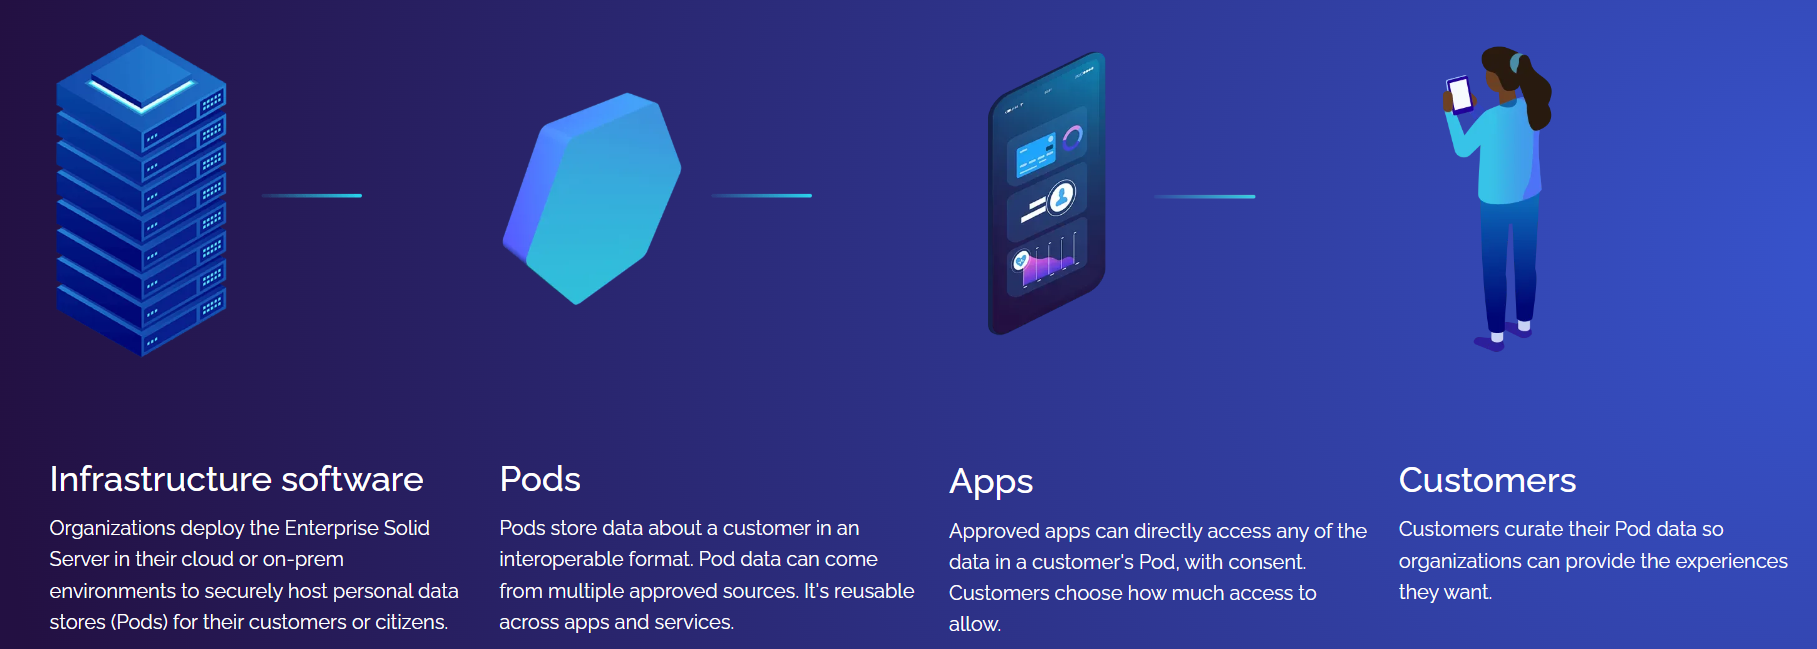
\includegraphics[width=\textwidth]{images/solid.png}
    \caption{Solid Framework \cite{solidImage}}
    \label{fig:solidImage}
\end{figure}

These pods are personal data stores that provide a place for both user and service provider to access and update data. This data can also be shared by the user with third party clients by granting them the necessary permission using the proposed third party authentication protocol called Solid OpenID Connect \cite{solidWebsite}. In short, this protocol uses the users consent to allow the service provider the distribution of a dpop token to a third party client, which grants access to private resources on the pod. However, a previous paper by Fett et al \cite{fett2016comprehensive} already discovered a potential mixup attack on OpenID Connect. As Solid OpenID Connect is based on OpenID Connect, the first goal of this paper is the search for a similar or even the same vulnerability in Solid OpenID Connect by creating a tool verifiable model.

\begin{mdframed}
1. The creation and verification of a model depicting Solid Open ID Connect. The criterion of the model was it to be sufficiently rich to demonstrate the presence of a suspected mixup attack.
\end{mdframed}

The second goal of the paper follows-up on the first goal: during the development of the model and its verification, two different attacks have been discovered. To prevent the attacks from being exploitable, a potential fix is modelled and verified. The resulting protocol is then proposed as a new version of SOIDC.

\begin{mdframed}
2. Proposition for a fixed version of SOIDC, nullifying the previously discovered attacks.
\end{mdframed}

The third and last goal of the paper addresses a common problem shared by third party authentication protocols: based on their particular architecture, the identity provider needs to learn about the resource being accessed before generating an access token. This allows them to track user behaviour and create profiles, which may be used to generate commercial profit. With the aim to increase the privacy of the user, this paper proposes a new form of protocol using verifiable credentials, leading to the identity provider losing the ability to track user behaviour and therefore increasing user privacy.

\begin{mdframed}
3. The creation and verification of a new protocol providing third party authentication using verifiable credentials.
\end{mdframed}

This paper is divided into the following parts: chapter \ref{proverif} presents the tool used in this paper to acquire proof for its security statements. Chapter \ref{soidc} takes a closer look at Solid Open ID Connect (SOIDC), a specification allowing users to grant access to third party services to private information stored on supervised servers. Chapter \ref{msoidc} is taking the main idea of SOIDC and mixing it with the idea of verifiable credentials to create a new protocol that provides more privacy for the user and protects their information from being tracked by the identity provider. Chapter \ref{limitations_work} addresses the limitations of this paper and gives some guidance for potential further work. Chapter \ref{summary} summarizes the most important aspects of the the paper. The appendix contains the models used to verify authentication properties, which were explained in the paper. These models may be used to recreate the verification proofs or as a starting point for future work.

% -----------------------------------------------------------------------------
% -----------------------------------------------------------------------------
% -----------------------------------------------------------------------------

\chapter{ProVerif}
\label{proverif}

In order to achieve the goals mentioned above, it is important to go beyond intuition and use a tool providing the capabilities needed to formally proof and disprove statements. The tool chosen for this paper is called ProVerif and was created by Bruno Blanchet et al. \cite{proverif}. It is a cryptographic protocol verifier using applied $\pi$-calculus to find solid evidence for different statements. It is capable of modelling many cryptographic primitives like both symmetric and asymmetric encryption, signatures and hash functions. Additionally, due to using well-chosen approximations, it is capable of handling an infinite number of sessions of the protocol, which may even run in parallel. These feats combined allow the verification of secrecy and authentication properties, which constitute the goal of this paper.

In regard to its trustworthiness, ProVerif states in its manual that it is sound, but not complete. In other words, in case a property is satisfied in the eyes of ProVerif, then the model does guarantee the property in question. In contrast, in case ProVerif is not finding a proof for a given property, the model may nonetheless provide that property. Being sound but not complete makes ProVerif an adequate choice for achieving the goal of this paper, as each verification result can be trusted \cite{proverifManual}.

ProVerif relies on the symbolic, Dolev-Yao model of cryptography. This means that is goes beyond a passive, eavesdropping attacker and assumes that the adversary is able to also read, modify, delay, delete and inject messages according to their current knowledge. Moreover, all models created in this paper are using an open network architecture, which makes it possible for the attacker to pose as any of the honest actors in each protocol. This mirrors the capabilities of attackers on the web, strengthening the models and their verification results even further. In the given models, each actor both has an identity, a secret and a matching public key, which may be used for asymmetric encryption and signatures. Identities and public keys are globally known, while the secret keys remain private. It is assumed that the attacker is not able to break any underlying cryptographic primitives like encryptions, reverse hashes or forge signatures.

% -----------------------------------------------------------------------------

\newpage
\section{General Model Structure}

The syntax of ProVerif is broad and provides a whole set of various operations, which may be used in many different ways. This makes it important to keep the models well structured to make grasping the underlying meaning as easy as possible. Therefore, all models in this paper are using a simple structure, which is briefly explained in the following. Complete models are also accessible in the appendix \ref{appendix}.

\subsection{Definitions}

Firstly, the model starts out with general definitions. As general cryptographic primitives are not immediately part of the syntax, they need to defined using functions and reductions. The following example illustrates the definition of symmetric encryption and decryption:

\begin{Verbatim}[fontsize=\small]
    fun enc(bitstring, SymmetricKey):bitstring.
    reduc forall msg:bitstring,symk:SymmetricKey; dec(enc(msg,symk),symk)=msg.
\end{Verbatim}

After declaring all relevant cryptographic primitives, the model needs variables. Constants are global variables, which may be used by both the attacker and the honest actors. Free variables are used to check the attackers access on different values, which are subsequently used in secrecy claim evaluation. Events are used to save message sets, which are subsequently used in authentication claim evaluation:

\begin{Verbatim}[fontsize=\small]
    const tag1:bitstring.
    free free_code: bitstring [private].
    event appSendsLastMessageToIssuer(bitstring, bitstring, bitstring).
\end{Verbatim}

\subsection{Agent Macros}

Right after the definitions come the actor declarations. Each actor participating in the protocol is listed here. This part may be seen as the core of the model, as it defines all messages being send from one actor to another. This implies that each message is appearing twice, as it must both be send as output by someone and read as input by someone else. The following example illustrates the message passing process between browser and app:

\begin{Verbatim}[fontsize=\small]
    (* Browser *)
    new n:bitstring;
    new sskI:SecretKey;
    let m_1 = aenc((tag1, n, pk(sskI)), pka) in
    out(c, m_1);

    (* App *)
    in(c, m_1:bitstring);
    let (tag1':bitstring, n:bitstring, spkI:PublicKey) = adec(m_1, ska) in
    if (tag1 = tag1') then
\end{Verbatim}

\subsection{Open Network}

At the current state, the model is only checking properties in regard to an attacker, who may easily be distinguished from the honest actors. In order to give the attacker more control, the open network part of the model allows them to pose as any actor. This mimics the capabilities of a real attacker on the internet and gives the model additional importance when verifying its properties. The open network of for instance an app may be modelled like this:

\begin{Verbatim}[fontsize=\small]
    let open_app(c:channel, a:bitstring, ska:SecretKey, u:bitstring, 
    pku:PublicKey, i:bitstring, pki:PublicKey) =
      in(c, e1:bitstring);
      in(c, e2:bitstring);
      if (e1 = u) && (e2 = i) then
        app(true, c, a, ska, u, pku, i, pki)
      else
      if (e1 <> u) && (e2 = i) then
        in(c, pke1:PublicKey);
        app(false, c, a, ska, e1, pke1, i, pki)
      else
      if (e1 = u) && (e2 <> i) then
        in(c, pke2:PublicKey);
        app(false, c, a, ska, u, pku, e2, pke2)
      else
      if (e1 <> u) && (e2 <> i) then
        in(c, pke1:PublicKey);
        in(c, pke2:PublicKey);
        app(false, c, a, ska, e1, pke1, e2, pke2)
      .
\end{Verbatim}

\subsection{Assumptions}

This part of the model defines the properties, which are checked by ProVerif. The simplest property to verify is secrecy of different free variables. It is used to establish if a protocol managed to successfully complete or if some important variable like a password remains secret:

\begin{Verbatim}[fontsize=\small]
    query attacker(check_reach_app).
    query attacker(free_password).
\end{Verbatim}

Furthermore, ProVerif is able to verify authentication claims using the previously explained event statements. In the following example, the claim states that an app may only complete its protocol when all messages it received match the messages send by the browser and issuer:

\begin{Verbatim}[fontsize=\small]
    query m_1:bitstring, m_2:bitstring, m_3:bitstring, m_8:bitstring, m_9:bitstring,
    m_10:bitstring, m_11:bitstring, m_12:bitstring;
        inj-event(appCompletesProtocol(m_1, m_2, m_3, m_8, m_9, m_10, m_11, m_12))
        ==>
        inj-event(browserSendsLastMessageToApp(m_1, m_2, m_3, m_8))
        &&
        inj-event(issuerSendsLastMessageToApp(m_9, m_10, m_11, m_12))
        .
\end{Verbatim}

\subsection{Main}

The main section of the model is the starting point of the ProVerif verification process. In this part, secret keys as well as public identities and keys are being created, before they are distributed to the different processes. The processes themselves are running in parallel and may be replicated any number of times. This mimics the attackers ability to start as many sessions as needed to find and exploit a vulnerability in the protocol:

\begin{Verbatim}[fontsize=\small]
    (* create identities *)
    new a:bitstring;
    new u:bitstring;
    new i:bitstring;

    (*advertise identities*)
    out(c,a);
    out(c,u);
    out(c,i);

    (*declare secret keys*)
    new ska:SecretKey;
    new sku:SecretKey;
    new ski:SecretKey;

    (*advertise public keys*)
    out(c,pk(ska));
    out(c,pk(sku));
    out(c,pk(ski));

    (*generate variables*)
    new password:bitstring;

    (*let agents dance*)
    (
        ! open_app      (c, a, ska, u, pk(sku), i, pk(ski))
      | ! open_browser  (c, u, sku, a, pk(ska), i, pk(ski), password)
      | ! open_issuer   (c, i, ski, a, pk(ska), u, pk(sku), password)
    )
\end{Verbatim}

% -----------------------------------------------------------------------------

\section{Encountered Problems}

This part of the paper mentions some of the most dominant problems slowing down the progress of the model creation and verification. For each iterated problem, a possible solution is given to facilitate further development.

\subsection{Bloating}
\label{proverif_bloating}

Unfortunately during the development of the model, an inherent weakness of ProVerif made the verification process slow and tedious. When verifying a protocol, it may occur that the existence of infinite loops prevent the process form finishing. These infinite loops may result from message structures of the following form:

\begin{flushleft}
    \hspace{2cm} $B \rightarrow A : s e n c (N_b, k )$ \\
    \hspace{2cm} $A \rightarrow B : s e n c ( f (N_b ) , k )$
\end{flushleft}

In order to find out the value of the nonce $N_b$, the attacker could take the second message $f (N_b $) and use it as an input to restart the sequence again, obtaining $f ( f (Nb))$. This could again be sent as the input of the first message, resulting in an infinite loop. Preventing this behaviour can be done by adding tags to the use of each cryptograhic primitive, like so:

\begin{flushleft}
    \hspace{2cm} $B \rightarrow A : s e n c ( ( c_0 , N_b ) , k )$ \\
    \hspace{2cm} $A \rightarrow B : s e n c ( ( c_1 , f (N_b ) ) , k )$
\end{flushleft}

With tags, the messages can't be mixed anymore, which enables the verification process to finish. However, when using tags in the verification process, they should also be used in the implementation of the protocol. The security of the tagged protocol does not imply the security of the untagged version \cite{proverifManual}.

\subsection{Identical Messages}

Another common problem which leads to unnecessary bloating during the verification process is the appearance of exactly the same messages in the same protocol. In this case, ProVerif is not able to reliably match the outputs with their corresponding inputs. Therefore, when having the requirement to use identical messages at different places in the model, it is advised to artificially change some part of them to support ProVerif in its verification process. This may be achieved by adding some constant or using some function, which is not changing anything essential to the protocol. Alternatively, if sending a tuple containing different types of terms, reordering them may also work and is good practice, as it prevents potential replay attacks.

\subsection{Non-Bitstring Messages}

During the development of the protocol, it appeared that using messages of any type other than bitstring leads to unforeseen behaviour, often resulting in ProVerif not being able to match outputs with corresponding inputs and therefore not being able to finish the verification of the protocol. One example of such an occurrence is the transmission of the first message in a Diffie Hellman key exchange. This message is an element of the group G raised by some exponent, resulting in another element of group G. Without first converting it to a bitstring using a custom function, ProVerif was not able to complete the protocol.

% -----------------------------------------------------------------------------
% -----------------------------------------------------------------------------
% -----------------------------------------------------------------------------

\chapter{Solid OpenID Connect}
\label{soidc}

Since the release of the OAuth 2.0 [RFC6749] and OpenID Connect Core 1.0 [OIDC.Core] web standards, they have quickly been adopted across the industry in various applications. These extended practical uses offered a lot of insight on their corresponding strengths through extensive real-world data and experience. However, with the growing importance of privacy and digital identities in our modernising world, an improvement was proposed. SOIDC aims at eliminating the previously necessary trust relationship between identity providers and resource servers including their corresponding authorisation servers \cite{solid}. This part of the paper analyses the message flow used to accomplish that goal by providing a verifiable model supporting the initial claims.

When taking a look at the SOIDC message flow described in their primer \cite{solidPrimer}, it is clearly divided in two different parts: the first part called 'Authorization Code Grant' and takes care of the access token distribution, while the second part is called 'Request Flow' and takes care of the token and resource exchange. After finishing the modelling and verification process of the first part, it became apparent that it already showed signs of major vulnerabilities. Therefore, this paper focuses its analysis on the first part, gaining in-depth knowledge about these vulnerabilities and providing a possible fix. The second part of SOIDC is not included in this process and may be analysed in future work.

% -----------------------------------------------------------------------------

\section{HTTPS Handshake}

\subsection{Simple vs Diffie Hellman}

When beginning to model Solid Open ID Connect, the first step is to search for a way to model a secure connection on the web using HTTPS. This kind of connection is characterized through its uni-directional authentication, usually granted to important servers using certificates from trusted third parties to acknowledge their specific public keys. These certificates may then be verified by the connecting browser to guarantee communication with the chosen party and not some imposter. The main goal of such a connection process is the establishment of a symmetric session key, which may be used for any further communication. This results in forward secrecy, which means that even the compromise of the long-term keys cannot result in a loss of secrecy of older communication sessions. The connecting party usually authenticates later in the process through some sort of shared secret, like for instance a password. One possibility of modelling a protocol providing these properties is depicted in the msc \ref{fig:msc_https}. It intentionally forgoes authentication for the initiator, highlighting the fact that anyone is able to connect anonymously to a certified web server. This protocol is verified using ProVerif and provides exactly the anticipated security factors: both parties are able to finish execution of the handshake and sharing a symmetric key. Even though only the initiator is able to authenticate the responder, no attacker is able to compromise the symmetric session key. 

\begin{figure}[H]
    \centering
    %\makebox[\textwidth][c]{

\begin{msc}[instance distance=6cm]{HTTPS Connect}

\declinst[instance width = 3cm]{initiator}{$pk(sk_r)$}{Initiator}
\declinst[instance width = 3cm]{responder}{$sk_r$}{Responder}

\action*{\small{new n: nonce}}{initiator}
\action*{\small{new symk: SymmetricKey}}{responder}
\nextlevel[2]
\action*{\small{new $sk_i$: SecretKey}}{initiator}
\nextlevel[2]
\mess{\small{$\{ n,pk(sk_i) \} pk(sk_r)$}}{initiator}{responder}
\nextlevel[2]
\mess{\small{$\{ n,symk \} pk(sk_i)$}}{responder}{initiator}
\nextlevel[1]
\condition*{\small{Auth. Responder}}{initiator}
\ncondition*{\small{Auth. Initiator}}{responder}
\nextlevel[1]

\end{msc}

%}
    \caption{HTTPS Connect}
    \label{fig:msc_https}
\end{figure}

Alternatively, a much stronger handshake mimicing HTTPS may be modelled by using a variation of the Diffie Hellman Key Exchange (DHKE) as depicted in the msc \ref{fig:msc_https_dh}. 

\begin{figure}[H]
    \centering
    % HTTPS is used to establish a session key, providing forward secrecy

%\makebox[\textwidth][c]{

\begin{msc}[instance distance=6cm]{HTTPS Connect Using Diffie Hellman}

\declinst[instance width = 3cm]{initiator}{$sk_I$, $pk(sk_R)$}{Initiator}
\declinst[instance width = 3cm]{responder}{$sk_R$, $pk(sk_I)$}{Responder}

\action*{\small{new x: exponent}}{initiator}
\action*{\small{new y: exponent}}{responder}
\nextlevel[2]
\action*{\small{$gx = g^x$}}{initiator}
\action*{\small{$gy = g^y$}}{responder}
\nextlevel[2]
\mess{\small{gx}}{initiator}{responder}
\nextlevel[2]
\mess{\small{gy, $\{sign((gy,gx),sk_R)\}_k$}}{responder}{initiator}
\nextlevel[1]
\action*{\small{k = $(gx)^{y}$}}{responder}
\action*{\small{k = $(gy)^{x}$}}{initiator}
\nextlevel[2]
\condition*{\small{Auth. Responder}}{initiator}
\ncondition*{\small{Auth. Initiator}}{responder}
\nextlevel[1]


\end{msc}

%}
    \caption{HTTPS Connect Using Diffie Hellman}
    \label{fig:msc_https_dh}
\end{figure}

As a standard DHKE is vulnerable to man in the middle attacks, the variation is using a signature to ensure the presence of the honest party and agreement on the same key material, preventing any attacker of inserting their own. Its strength comes from the fact that, in contrast to the previous protocol, both parties add partial information to a combined symmetric session key. This denies the capability of an attacker to pose as an honest party and to decide on the session key themselves. This protocol is verified using ProVerif and provides the exact same qualities as the previous handshake proposal. However, even tough this version is stronger, it puts a lot more strain on ProVerif when verifying the entire authorization code grant explained in the next section. 

\subsection{Timing Results}

Verifying the simple HTTPS variant is fast with verification times generally below 5 minutes. In contrast, verifying the Diffie Hellman variant harbours some bloating problems as explained in section \ref{proverif_bloating}. This leads to long verification times, even with the use of tags already mitigating the problem. The following tables show in detail the verification results of SOIDC using the simple version in comparison with the Diffie Hellman version:

    \begin{table}[H]
        \centering
        \def\arraystretch{1.5}
        \resizebox{0.9\textwidth}{!}{
        \begin{tabular}{ | l | l | l | l | }
             \hline
             \multicolumn{4}{|l|}{Solid Open ID Connect}\\
             \hline
             Property & Holds in Simple & Holds in DH & Verification Time DH \\ 
             \hline
              Auth. App & Yes & Yes & 1h15 \\
              Auth. Browser & Yes & Yes & 1h15 \\
              Auth. Issuer & No & \color{purple}OOM\color{black} & 2h15 (2.553 rules) \\
             \hline
        \end{tabular}}
    \end{table}

    \begin{table}[H]
        \centering
        \def\arraystretch{1.5}
        \resizebox{0.9\textwidth}{!}{
        \begin{tabular}{ | l | l | l| l | }
             \hline
             \multicolumn{4}{|l|}{Solid Open ID Connect With Fix}\\
             \hline
             Property & Holds in Simple & Holds in DH & Verification Time DH \\ 
             \hline
              Auth. App & Yes & Yes & 0h30 \\
              Auth. Browser & Yes & Yes & 0h30 \\
              Auth. Issuer & Yes & Yes & 1h30 \\
             \hline
        \end{tabular}}
    \end{table}

As seen above, ProVerif is not capable of finding the issuer mixup attack when using the DH handshake, as it runs out of memory with 2.553 rules in queue. Even though this amount of rules is quite low, it can always happen that it bloats up again in the course of verification. The DH version with fix finished as expected. The following tables show in detail the verification results of SOIDC with a late handshake using the simple version in comparison with the Diffie Hellman version:

    \begin{table}[H]
        \centering
        \def\arraystretch{1.5}
        \resizebox{0.9\textwidth}{!}{
        \begin{tabular}{ | l | l | l| l | }
             \hline
             \multicolumn{4}{|l|}{Solid Open ID Connect Late HS}\\
             \hline
             Property & Holds in Simple & Holds in DH & Verification Time DH \\ 
             \hline 
              Auth. App & No & \color{purple}OOM\color{black} & 0h45 (7.060 rules) \\
              Auth. Browser & Yes & \color{purple}OOM\color{black} & 1h00 (29.496 rules) \\
              Auth. Issuer & No & \color{purple}OOM\color{black} & 1h15 (12.763 rules) \\
             \hline
        \end{tabular}}
    \end{table}

    \begin{table}[H]
        \centering
        \def\arraystretch{1.5}
        \resizebox{0.9\textwidth}{!}{
        \begin{tabular}{ | l | l | l| l | }
             \hline
             \multicolumn{4}{|l|}{Solid Open ID Connect Late HS With Fix}\\
             \hline
             Property & Holds in Simple & Holds in DH & Verification Time DH \\ 
             \hline
              Auth. App & Yes & Yes & 0h10 \\
              Auth. Browser & Yes & Yes & 0h10 \\
              Auth. Issuer & Yes & Yes & 0h10 \\
             \hline
        \end{tabular}}
    \end{table}

As seen above, Proverif is again not capable of finding the attack when using the DH handshake, as it runs out of memory with thousands of rules in queue. However, the fixed version is verified and running fast with a verification time of 10 minutes. Without ProVerif being able to identify the attacks on SOIDC using the Diffie Hellman handshake, this paper uses the previously explained simpler but weaker version in the following analysis.

% -----------------------------------------------------------------------------

\section{Authorization Code Grant Protocol}

As mentioned before, the authorization code grant protocol is taking care of app authentication and the following access token distribution. The model of the protocol in question is based on the message flow provided in the official Solid OIDC Primer \cite{solidPrimer} and is depicted in the msc \ref{fig:msc_soidc}. Some of the major model design choices are explained in the following, starting with its actors:

\textbf{App} - The App constitutes the relying party (RP) in the process, needing permission of the Resource Owner (RO) to access private information. 

\textbf{Browser} - The Browser of the RO is used to connect both App and Issuer, allowing them to talk via HTTPS requests. It also allows the RO to provide the needed password for the OpenID Provider (OP).

\textbf{Issuer} - The Issuer is the OP, providing the RP with the needed access token for the private resource if authentication succeeds.

After having declared the actors and their corresponding roles, the model skips the first few steps enumerated in the primer and supposes them to already be done. These steps include the 'Retrieve Profile' and the 'Retrieve OP Configuration' step, which are mainly used to setup communication between RP and OP. Additionally, the 'Fetch Client ID Document' step is skipped, as we suppose the OP already knows everything it needs without an attacker being able to interfere in this request.

Before starting communication and sending any message, the two actors in question are always using an HTTPS handshake to establish a connection. As previously mentioned, these handshakes are fashioned in a special way to only grant uni-lateral authentication. The little arrow in the msc \ref{fig:msc_soidc} indicates which party is actually authenticated. Using the HTTPS handshake before every communication between two parties also mimics the use of callbacks to communicate, as the generated session keys tightly bind messages together.

\begin{figure}[H]
    \centering
    %\makebox[\textwidth][c] {

\begin{msc}[environment distance = 3cm]{Solid Open ID Connect - Authorization Code Grant}

\declinst[instance width = 4cm]{app}{$sk_{A}$, pk($sk_I$)}{App}
\declinst[instance width = 4cm]{browser}{pk($sk_A$), pk($sk_I$), password}{Browser}
\declinst[instance width = 4cm]{issuer}{$sk_I$, password}{Issuer}

\condition*{\small{($\leftarrow$) $k_1$ = HTTPS Connect}}{app,browser}
\nextlevel[2]
\action*{\small{fresh pkce: nonce}}{app}
\nextlevel[3]
\mess{\small{$\{appID,h(pkce), scope\}_{k_1}$}}{app}{browser}
\nextlevel[1]
\condition*{\small{$k_2$ = HTTPS Connect ($\rightarrow$)}}{issuer,browser}
\nextlevel[3]
\mess{\small{$\{appID,h(pkce),scope,browserID,password\}_{k_2}$}}{browser}{issuer}
\nextlevel[1]
\action*{\small{fresh code: nonce}}{issuer}
\nextlevel[2]
\mess{\small{$\{code\}_{k_2}$}}{issuer}{browser}
\nextlevel[2]
\mess{\small{$\{code\}_{k_1}$}}{browser}{app}
\nextlevel[1]
\stop*{browser}
\nextlevel[1]
\condition*{\small{$k_3$ = HTTPS Connect ($\rightarrow$)}}{app,issuer}
\nextlevel[2]
\action*{\small{fresh sks: SecretKey, jti: nonce}}{app}
\nextlevel[3]
%\action*{\small{$T_2 = (appID, jti, code, pkce')$}}{app}
%\nextlevel[3]
\mess{\small{$\{pk(sks), sign((appID, jti, code, pkce), sks)\}_{k_3}$}}{app}{issuer}
\nextlevel[1]
\action*{\small{jtk = h(pk(sks))}}{issuer}
\nextlevel[3]
%\action*{\small{M = (jtk,jti,scope,appID,issuerID,browserID)}}{issuer}
%\nextlevel[3]
\mess{\small{$\{sign((jtk,jti,scope,appID,issuerID,browserID), skI)\}_{k_3}$}}{issuer}{app}
\nextlevel[1]

\end{msc}

%}
    \caption{SOIDC}
    \label{fig:msc_soidc}
\end{figure}

The first message actually being send is the authorisation request containing the appID, hashed pkce and scope. The appID is like the two other IDs a unique identifier for the app, the browser and the issuer respectively. Pkce is a generated code used by the app, which has the purpose to later guarantee the issuer that it is talking to the right app. The scope is related to the resource which is to be requested. Following the path over the browser, the RO is able to check on the values provided and login in case everything is valid. After receiving the values and checking them, the OP is generating a code which is send via the browser to the RP. This mimics SOIDCs send code to redirect uri step. Afterwards, the RP is using the code to request a dpop token, which can later be used for resource access. The request is mainly secured by a signature with a fresh generated key, as well as the pkce and the code from before. After checking the given information, the OP is issuing the requested token to the RP.

Verifying the model in ProVerif revealed that not every aspect of the model is secure. While the password stays secret throughout the entire protocol, the code is leaked to the attacker at some point. Further investigations revealed that not all parties are being authenticated correctly. The issuer in this case is not able to authenticate the app and the browser, meaning that there is a way the issuer finishes the protocol while talking to some entity pretending to either be app and / or browser. As this constitutes a serious vulnerability, the attack is explored in-depth in the next section of the paper. This completes the first goal of the paper as described in chapter \ref{introduction}.

\subsection{Mixup Attack for OpenID Provider}

\begin{figure}[H]
    \centering
    %\makebox[\textwidth][c] {

\begin{msc}[environment distance = 3cm]{Solid Open ID Connect - Attack on Issuer Authentication}

\declinst[instance width = 3cm]{app}{$sk_{A}$, pk($sk_E$)}{App}
\declinst[instance width = 3cm]{browser}{pk($sk_A$), pk($sk_I$), password}{Browser}
\dummyinst[instance width = 3cm]{eve}
\declinst[instance width = 3cm]{issuer}{$sk_I$, password}{Issuer}

\mess{\small{$\{n, pk(sskI)\}_{pk(ska)}$}}{browser}{app}
\nextlevel[2]
\mess{\small{$\{n, k_1\}_{pk(sskI)}$}}{app}{browser}
\nextlevel[2]
\mess{\small{$\{appID,h(pkce),scope\}_{k_1}$}}{app}{browser}
\nextlevel[1]
\mess{\small{$\{n_2, pk(sskI_2)\}_{pk(ski)}$}}{browser}{issuer}
\nextlevel[2]
\mess{\small{$\{n_2, k_2\}_{pk(sskI_2)}$}}{issuer}{browser}
\nextlevel[2]
\mess{\small{$\{appID,h(pkce),scope,browserID,password\}_{k_2}$}}{browser}{issuer}
\nextlevel[2]
\mess{\small{$\{code\}_{k_2}$}}{issuer}{browser}
\nextlevel[1]
\mess{\small{$\{code\}_{k_1}$}}{browser}{app}
\nextlevel[1]
\stop*{browser}
\nextlevel[1]
\startinst{eve}{$sk_{E}$, pk($sk_I$)}{Eve as Issuer / App}
\nextlevel[2]
\mess{\small{$\{n_3, pk(sskI3)\}_{pk(sk_{E})}$}}{app}{eve}
\nextlevel[2]
\mess{\small{$\{n_4, pk(sk_2)\}_{pk(ski)}$}}{eve}{issuer}
\nextlevel[2]
\mess{\small{$\{n_4, k_3\}_{pk(sk_2)}$}}{issuer}{eve}
\nextlevel[1]
\mess{\small{$\{n_3, k_3\}_{pk(sskI3)}$}}{eve}{app}
\nextlevel[2]
\mess{\small{$\{pk(sks), sign((appID, jti, code, pkce), sks)\}_{k_3}$}}{app}{eve}
\mess*{}{eve}{issuer}
\nextlevel[2]
\mess{\small{$\{sign((jtk,jti,scope,appID,issuerID,browserID), skI)\}_{k_3}$}}{issuer}{eve}
\nextlevel[1]

\end{msc}

%}
    \caption{SOIDC Attack On Issuer Authentication}
    \label{fig:msc_soidc_attack}
\end{figure}

In general, a mixup attack is a form of attack on a protocol, where the attacker Eve poses as one or more different agents to trick an honest party in sending sensitive information to them. This information may subsequently be used by Eve to perform usually restricted actions or get access to private information. Searching for such an attack in the model illustrating the authorisation code grant message flow, ProVerif revealed the attack depicted in the msc \ref{fig:msc_soidc_attack}. The complete model of this protocol is available in the appendix \ref{appendix_issuer_mixup}.

In the first steps of the attack, Eve is not acting at all and lets the app receive the the issuer generated code following the usual protocol. However, Eve then poses as a fake issuer in such a way, that the app starts performing the HTTPS handshake with them. Halfway through the handshake, Eve then connects to the real issuer, posing as the honest app. By cleverly mixing the handshakes, Eve is able to generate the same session key $k_3$ for both communication channels. After receiving the token request with code and code verifier from the honest app, Eve proceeds to forward this message to the honest issuer. This leads to the issuer assuming that Eve must be the honest app and proceeding to send them the access token, giving her access to private resources. The occurrence of such an attack may be tracked down to the simple fact that the app is not aware of the issuerID corresponding to the honest issuer. This problem is later addressed in the section \ref{fix_short}.

% -----------------------------------------------------------------------------

\subsection{Cross-Site Request Forgery}

In general, Cross-Site Request Forgeries (CSRF) aim at inducing users to perform actions they don't intend to perform. This includes actions like changing the password, changing their email address or sending money to somebody else. CSRF attacks only work if there is a relevant action to perform by the victim (like a password change), matching messages to the right session is handled by cookies and the hyperlink in question includes no parameter which is unknown to the attacker \cite{csrf}. Figure \ref{fig:csrf} depicts the general structure of such an attack.

\begin{figure}[H]
    \centering
    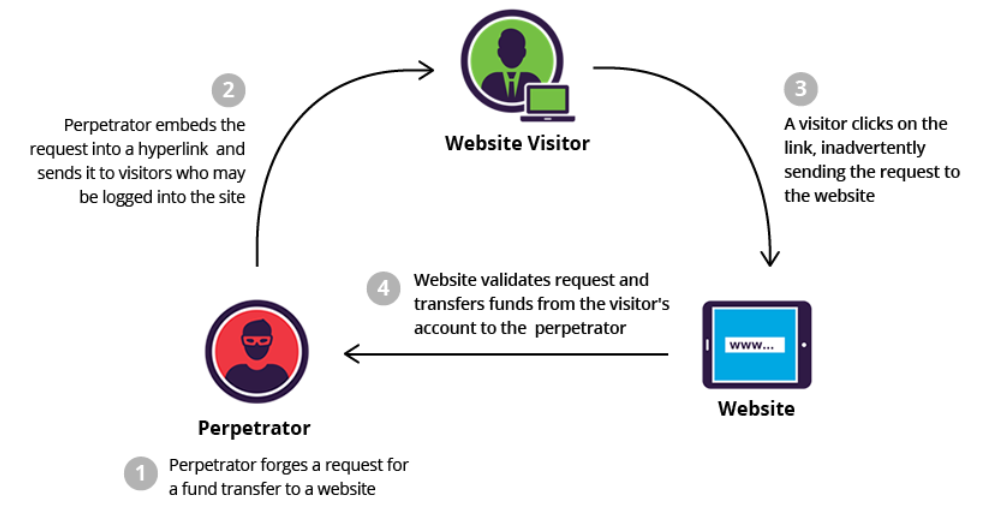
\includegraphics[width=\textwidth]{images/csrf.png}
    \caption{CSRF \cite{csrfImage}}
    \label{fig:csrf}
\end{figure}

Even though the original model illustrating the authorisation code grant message flow does not allow for this kind of attack, it is important to note that implementation errors may occur. Such errors may lead to delayed authentication, which may be modelled by shifting the handshakes like depicted in msc \ref{fig:msc_soidc_lateHS}, giving the attacker control over the initial authorisation request and allowing them to freely choose the values appID, pkce and scope. The complete model of this protocol is available in the appendix \ref{appendix_csrf}.

\begin{figure}[H]
    \centering
    %\makebox[\textwidth][c] {

\begin{msc}[environment distance = 3cm]{Solid Open ID Connect - Late HS}

\declinst[instance width = 4cm]{app}{$sk_{A}$, pk($sk_I$)}{App}
\declinst[instance width = 4cm]{browser}{pk($sk_A$), pk($sk_I$), password}{Browser}
\declinst[instance width = 4cm]{issuer}{$sk_I$, password}{Issuer}

\action*{\small{fresh pkce: nonce}}{app}
\nextlevel[3]
\mess{\small{$appID,h(pkce),scope$}}{app}{browser}
\nextlevel[1]
\condition*{\small{$k_2$ = HTTPS Connect ($\rightarrow$)}}{issuer,browser}
\nextlevel[3]
\mess{\small{$\{appID,h(pkce),scope,browserID,password\}_{k_2}$}}{browser}{issuer}
\nextlevel[1]
\action*{\small{fresh code: nonce}}{issuer}
\nextlevel[2]
\mess{\small{$\{code\}_{k_2}$}}{issuer}{browser}
\nextlevel[2]
\condition*{\small{($\leftarrow$) $k_1$ = HTTPS Connect}}{app,browser}
\nextlevel[3]
\mess{\small{$\{code\}_{k_1}$}}{browser}{app}
\nextlevel[1]
\stop*{browser}
\nextlevel[1]
\condition*{\small{...}}{app,issuer}
\nextlevel[2]

\end{msc}

%}
    \caption{SOIDC Late Handshake}
    \label{fig:msc_soidc_lateHS}
\end{figure}

Running a ProVerif verification on this model reveals the now existing CRSF attack, which emerged as the app is no longer authenticating browser and issuer. This leads again to the code to be leaked to the attacker, which in combination with the ability of choosing the authorisation request themselves, gives them free hand in using it with an honest issuer and acquiring an access token. This attack is depicted in msc \ref{fig:msc_soidc_lateHS_attack}.

\begin{figure}[H]
    \centering
    %\makebox[\textwidth][c] {

\begin{msc}[environment distance = 3cm]{Solid Open ID Connect - CSRF Attack}

\declinst[instance width = 3cm]{app}{$sk_{A}$, pk($sk_E$)}{App}
\declinst[instance width = 3cm]{browser}{pk($sk_A$), pk($sk_I$), password}{Browser}
\dummyinst[instance width = 3cm]{eve}
\declinst[instance width = 3cm]{issuer}{$sk_I$, password}{Issuer}

\mess{\small{$appID,h(pkce),scope$}}{app}{browser}
\nextlevel[2]
\mess{\small{$\{n_2, pk(sskI_2)\}_{pk(ski)}$}}{browser}{issuer}
\nextlevel[2]
\mess{\small{$\{n_2, k_2\}_{pk(sskI_2)}$}}{issuer}{browser}
\nextlevel[2]
\mess{\small{$\{appID,h(pkce),scope,browserID,password\}_{k_2}$}}{browser}{issuer}
\nextlevel[2]
\mess{\small{$\{code\}_{k_2}$}}{issuer}{browser}
\nextlevel[1]
\mess{\small{$\{n, pk(sskI)\}_{pk(ska)}$}}{browser}{app}
\nextlevel[2]
\mess{\small{$\{n, k_1\}_{pk(sskI)}$}}{app}{browser}
\nextlevel[2]
\mess{\small{$\{code\}_{k_1}$}}{browser}{app}
\nextlevel[2]
\stop*{browser}
\nextlevel[1]
\startinst{eve}{$sk_{E}$}{Eve as Issuer}
\nextlevel[2]
\mess{\small{$\{n_3, pk(sskI2)\}_{pk(sk)}$}}{app}{eve}
\nextlevel[2]
\mess{\small{$\{n_3, k_3\}_{pk(sskI2)}$}}{eve}{app}
\nextlevel[2]
\mess{\small{$\{pk(sks), sign((appID, jti, code, pkce), sks)\}_{k_3}$}}{app}{eve}
\nextlevel[2]
%\mess*{}{eve}{issuer}
%\nextlevel[2]
%\mess{\small{$\{sign((jtk,jti,scope,appID,issuerID,browserID), skI)\}_{k_3}$}}{issuer}{eve}
%\nextlevel[1]

\end{msc}

%}
    \caption{SOIDC CSRF Attack On Late Handshake}
    \label{fig:msc_soidc_lateHS_attack}
\end{figure}

% -----------------------------------------------------------------------------

\subsection{Providing a Fix}
\label{fix_short}

Being prone to such devastating attacks is indeed troublesome, but luckily both attacks rely on the same vulnerability and may be fixed easily. While the browser is talking to the issuer, the app has no way of knowing which issuer the browser is actually talking to. This may lead to misunderstandings, which may be exploited by malicious parties. However, by adding the issuerID to the code like shown in the msc \ref{fig:msc_soidc_fix_small}, the app learns about the identity of the conversing issuer. In case the identity is not matching with the apps expectation, the protocol can now be stopped, preventing sensitive information from leaking.

\begin{figure}[H]
    \centering
    %\makebox[\textwidth][c] {

\begin{msc}[environment distance = 3cm]{Solid Open ID Connect - Mixup Fix Proposal}

\declinst[instance width = 4cm]{app}{$sk_{A}$, pk($sk_I$)}{App}
\declinst[instance width = 4cm]{browser}{password}{Browser}
\declinst[instance width = 4cm]{issuer}{$sk_I$, pk($sk_{A}$), password}{Issuer}

\condition*{\small{...}}{app,browser,issuer}
\nextlevel[2]
\action*{\small{fresh code: nonce}}{issuer}
\nextlevel[3]
\mess{\small{$\{code, \color{purple}issuerID\color{black}\}_{k_2}$}}{issuer}{browser}
\nextlevel[1]
\mess{\small{$\{code, \color{purple}issuerID\color{black}\}_{k_1}$}}{browser}{app}
%\mess{\small{$code$, \color{purple}issuerID\color{black}}}{browser}{app}
\nextlevel[1]
\condition*{\small{...}}{app,browser,issuer}
\nextlevel[1]

\end{msc}

%}
    \caption{SOIDC Proposed Fix}
    \label{fig:msc_soidc_fix_small}
\end{figure}

Using ProVerif to verify the fix, it is proven that authentication now holds for all parties. This was tested for both the normal version and the version including the implementation error with the late handshake. Additionally, the code stays now secret throughout the entire run of the protocol. This denies both of the attacks mentioned beforehand. The following short snippet of ProVerif code illustrates the simplicity of the fix, as only two messages needed to be changed:

\begin{Verbatim}[fontsize=\small]
    (* ---------- Issuer ---------- *)
    (* Message 7 *)
    new code:bitstring;
    let m_7 = enc((tag7, code, i), k2) in
    event issuerSendsLastMessageToUser(m_4, m_5, m_6, m_7);
    out(c, m_7);

    (* ---------- User ---------- *)
    (* Message 7 *)
    in(c, m_7:bitstring);
    let (tag7':bitstring, code:bitstring, i':bitstring) = dec(m_7, k2) in
    if (tag7 = tag7') then
    if (i = i') then

    (* Message 8 *)
    let m_8 = enc((tag8, code, i), k1) in
    event browserSendsLastMessageToApp(m_1, m_2, m_3, m_8);
    out(c, m_8);

    (* ---------- App ---------- *)
    (* Message 8 *)
    in(c, m_8:bitstring);
    let (tag8':bitstring, code:bitstring, i':bitstring) = dec(m_8, k1) in
    if (tag8 = tag8') then
    if (i = i') then
\end{Verbatim}

Furthermore, applying the fix also allows for the pkce to be completely be omitted without losing security, as it is no longer the sole responsible for issuer authentication. 

% -----------------------------------------------------------------------------

\subsection{Proposed Version Of SOIDC}

A new and improved version of the SOIDC authorisation code grant protocol is proposed in the following and depicted in the msc \ref{fig:msc_soidc_fix}. It utilizes the fix proposed in section \ref{fix_short} and has had the code verifier pkce removed as it became obsolete in the process. Running the verification process of ProVerif on this model proved that authentication now holds for each party. Additionally, the code stays secret throughout the entire protocol. This completes the second goal of the paper as described in chapter \ref{introduction}.

\begin{figure}[H]
    \centering
    %\makebox[\textwidth][c] {

\begin{msc}[environment distance = 3cm]{Solid Open ID Connect - Authorization Code Grant Proposed Fix}

\declinst[instance width = 4cm]{app}{$sk_{A}$, pk($sk_I$)}{App}
\declinst[instance width = 4cm]{browser}{pk($sk_A$), pk($sk_I$), password}{Browser}
\declinst[instance width = 4cm]{issuer}{$sk_I$, password}{Issuer}

\condition*{\small{($\leftarrow$) $k_1$ = HTTPS Connect}}{app,browser}
\nextlevel[3]
\mess{\small{$\{appID, scope\}_{k_1}$}}{app}{browser}
\nextlevel[1]
\condition*{\small{$k_2$ = HTTPS Connect ($\rightarrow$)}}{issuer,browser}
\nextlevel[3]
\mess{\small{$\{appID,scope,browserID,password\}_{k_2}$}}{browser}{issuer}
\nextlevel[1]
\action*{\small{fresh code: nonce}}{issuer}
\nextlevel[3]
\mess{\small{$\{code, issuerID\}_{k_2}$}}{issuer}{browser}
\nextlevel[2]
\mess{\small{$\{code, issuerID\}_{k_1}$}}{browser}{app}
\nextlevel[1]
\stop*{browser}
\nextlevel[1]
\condition*{\small{$k_3$ = HTTPS Connect ($\rightarrow$)}}{app,issuer}
\nextlevel[2]
\action*{\small{fresh sks: SecretKey, jti: nonce}}{app}
\nextlevel[3]
%\action*{\small{$T_2 = (appID, jti, code)$}}{app}
%\nextlevel[3]
\mess{\small{$\{pk(sks), sign((appID, jti, code), sks)\}_{k_3}$}}{app}{issuer}
\nextlevel[1]
\action*{\small{jtk = h(pk(sks))}}{issuer}
\nextlevel[3]
%\action*{\small{M = (jtk,jti,scope,appID,issuerID,browserID)}}{issuer}
%\nextlevel[3]
\mess{\small{$\{sign((jtk,jti,scope,appID,issuerID,browserID), skI)\}_{k_3}$}}{issuer}{app}
\nextlevel[1]

\end{msc}

%}
    \caption{SOIDC Proposed Fixed Version}
    \label{fig:msc_soidc_fix}
\end{figure}

% -----------------------------------------------------------------------------
% -----------------------------------------------------------------------------
% -----------------------------------------------------------------------------

\chapter{New VC-Based Third Party Authentication Protocol}
\label{msoidc}

After having analysed and modelled the inner workings of Solid Open ID Connect, it becomes clear that relying on HTTPS connection protocols is not enough for the creation of secure communication channels. The existence of the previously discovered mixup and CSRF attacks prove the lack of control over the participants of the protocol. In order to regain control, the use of a bi-directional authenticating protocol is therefore proposed and modelled in the following. This should order the chaotic message flow jumping between all actors and provide less opportunities for a malicious party to infiltrate the system. 

Additionally, the protocol flow of Solid Open ID Connect implies that the issuer contacted every time a user grants a third party access to private resources. The third party in question is therefore transmitted to the issuer, allowing them to create profiles and track user behaviour based on that information. Reclaiming that privacy may be achieved by circumventing the need for the issuer to know the third party. To achieve this feat, the concept of Verifiable Credentials (VC) is introduced in the following. In general, VCs are official documents issued by an authority, proving that an entity is indeed fulfilling some sort of requirement. They are the digital counterpart of for instance a passport or identity card, which are issued by the government and proving the holder's name, age etc. By transferring this system to a third party authentication protocol, it becomes possible for any user to provide trustworthy evidence to a third party, which allows them to access sensitive information on their behalf. By adding an expiry date, these credentials may be used multiple times before they need to be refreshed by issuer \cite{credentials}.

% -----------------------------------------------------------------------------

\section{STS Handshake}

Similar to the HTTPS connection protocol mentioned in chapter \ref{soidc}, the Station To Station (STS) Protocol \cite{o1987encryption} aims at establishing a symmetric session key, which may be used for communication while providing forward secrecy. It is based on a Diffie Hellman Key Exchange operating in a previously fixed group G. Both parties start by exchanging a group element, which is raised by individually created secret exponents. As only the result is transferred, no attacker is able to identify the secret exponent. By raising the received group element again by their individual exponents, both parties now obtain the same group element, which may be used as a symmetric key for future communication. 

\begin{figure}[H]
    \centering
    \begin{msc}[instance distance=6cm]{STS Key Exchange}

\declinst[instance width = 3cm]{initiator}{$sk_I$, $pk(sk_R)$}{Initiator}
\declinst[instance width = 3cm]{responder}{$sk_R$, $pk(sk_I)$}{Responder}


\action*{\small{new x: exponent}}{initiator}
\action*{\small{new y: exponent}}{responder}
\nextlevel[2]
\action*{\small{$gx = g^x$}}{initiator}
\action*{\small{$gy = g^y$}}{responder}
\nextlevel[2]
\mess{\small{gx}}{initiator}{responder}
\nextlevel[2]
\mess{\small{gy, {sign((gy,gx),$sk_R$)}}}{responder}{initiator}
\nextlevel[2]
\mess{\small{sign((gx,gy),$sk_I$)}}{initiator}{responder}
\nextlevel[2]
\action*{\small{k = $(gx)^{y}$}}{responder}
\action*{\small{k = $(gy)^{x}$}}{initiator}
\nextlevel[2]
\condition*{Auth. Responder}{initiator}
\condition*{Auth. Initiator}{responder}
\nextlevel[2]

\end{msc}
    \caption{STS Connect}
    \label{fig:msc_sts}
\end{figure}

In general, this process is prone to a man in the middle attack. However, this is prevented by using signatures from both communicating parties to agree on the key material, also binding the generated symmetric key to their session. This process is illustrated in msc \ref{fig:msc_sts}. Verifying the protocol with ProVerif reveals that both parties are authenticating each other like anticipated. Additionally, the generated symmetric key stays secret throughout the entire protocol. 

% -----------------------------------------------------------------------------

\section{VC Issuance and Use}

By cooperating with Christoph Braun from the Karlsruhe Institute of Technology (KIT), a first version of a VC-based third party authentication protocol has been created. All of his work on this topic is accessible in the corresponding GitHub repository \cite{githubChristoph}, while this paper shows a slightly modified version based on the result of our collaboration. The main difference is the use of expanded attacker capabilities by using the open network model as explained in chapter \ref{proverif}, as it allows the attacker to pose as any party involved in the communication process. The protocol is divided into two different parts: The issuance of the VC by the issuer and its use to access private resources in a pod. Both parts are divided by a fictive sovereignty line, depicting the breaking point at which the issuer loses sight of the users targeted pod, thus increasing their privacy. The entire protocol is depicted in msc \ref{fig:msc_msoidc_small}, while both individual parts are explained in further detail in the following. The complete model of this protocol is available in the appendix \ref{appendix_msoidc}.

\begin{figure}[H]
    \centering
    

%\makebox[\textwidth][c]{

\begin{msc}[instance distance=1.6cm]{VC Issuance and Use}

\declinst[instance width = 3cm]{issuer}{$ski$, $pki$, $pku$, password}{Issuer}
\declinst[instance width = 3cm]{user}{$sku$, $pku$, $pka$, solid}{User}
\declinst[instance width = 3cm]{pod}{$skp$, $pkp$, $pka$}{Pod}


\condition*{\small{$k_1$ = STS Key Exchange}}{user,issuer}
\nextlevel[3]
\mess{\small{$\{u, attr, password\}_{k_1}$}}{user}{issuer}
\nextlevel[1]
\condition*{\small{if u / attr / pw valid}}{issuer}
\nextlevel[2]
\action*{\small{claims = ($u,i,attr$)}}{issuer}
\nextlevel[2]
\action*{\small{$VC = (claims, sig(claims, ski)$}}{issuer}
\nextlevel[3]
\mess{\small{$\{sig((VC),ski)\}_{k_1}$}}{issuer}{user}


\nextlevel[2]
%\msccomment[msccomment distance = 14cm]{sovereignity line}{issuer}
\settimer[]{sovereignity line}{issuer}
\order[pos = 2]{pod}{user}
\order[pos = 2]{user}{issuer}
\nextlevel[1]


\condition*{\small{$k_2$ = STS Key Exchange}}{user,pod}
\nextlevel[2]
\action*{\small{N = (VC, scope, solid)}}{user}
\nextlevel[2]
\action*{\small{PT = sig(N,sku)}}{user}
\nextlevel[2]
\mess{\small{$\{uri\}_{k_2}$}}{user}{pod}
\nextlevel[2]
\mess{\small{$\{rule\}_{k_2}$}}{pod}{user}
\nextlevel[2]
\mess{\small{$\{PT\}_{k_2}$}}{user}{pod}
\nextlevel[2]
\mess{\small{$\{sig((accesstoken), skp)\}_{k_3}$}}{pod}{user}
\nextlevel[2]


\end{msc}

%}
    \caption{VC Issuance and Use}
    \label{fig:msc_msoidc_small}
\end{figure}

The first part of the proposed protocol consists in acquiring a verifiable credential from an official issuer. After connecting to the issuer in question, the user is sending their identifier u, some sort of attribute they want to be certified and a previously established password. The methods used to agree an a password are not included in this model. Each of the previously send terms fulfills a different role: The user identifier determines whose attribute should be approved by the issuer. The attribute determines what should be approved, like for instance a university degree or similar. The password is authenticating the user. After verifying the given information, the issuer creates a verifiable credential (VC) by signing the user identifier, their own identifier and the attribute in question. This provides solid proof that the claim has been seen, verified and accorded by the issuer.

The second part of the proposed protocol starts below the sovereignty line and consists in the creation and use of the presentation token (PT) to get access to a specific resource. Transforming the VC to a PT by signing it is only possible for the user and is an important step as the holder of a VC is able to grant third party access to resources. Transferring the raw VC to any other party allows them to distribute access to private resources and thus should be avoided at all cost. In contrast, the possession of the PT only grants access to the resource specified in the scope and does not allow further distribution as it is already signed by the user. The next step consists in sending the resource access request uri to the pod. After receiving the request, the permission server is exposing the rule needed to fulfill in order to access the resource in question. The rule could for instance be the requirement of being registered on a specific website. With the matching PT, the app is able to provide proof of respecting the rule. Afterwards, the app receives an access token, which may be used to access the resource initially requested, completing the protocol.

The protocol was modelled and verified in ProVerif. The verification confirms that each party is able to complete the protocol and that both symmetric communication keys and the password stay secret during that time. Additionally, each actor is able to authenticate each other actor, meaning that no mixup attacks are possible in this scenario. This completes the third goal of the paper as described in chapter \ref{introduction}.

% -----------------------------------------------------------------------------
% -----------------------------------------------------------------------------
% -----------------------------------------------------------------------------

\chapter{Limitations / Further Work}
\label{limitations_work}

Even though the models provided in this paper are as detailed as possible, it is important to make a note on the natural limitations of a model. These limitations emerge a model is in general not able to represent reality in its entirety. They usually use a set of assumptions, which aim at reducing the cheer amount of possibilities occurring in real life. If not chosen carefully, it may happen that some important aspects are abstracted away, hiding the potential existence of other attacks. That said, models are still a strong tool and should be used as much as possible during the creation process of any protocol. Each time a model is finding an attack, the discovered attack may be prevented before any malicious party is capable of exploiting it. This already protects user data even during development of a new protocol. Additionally, providing models and verification as proof for attacks or security properties is a guarantee for their existence.

When continuing the work on verifying Solid OpenID Connect, the next step would be to create a model illustrating its second part called 'Request Flow' as described in the official Solid Primer \cite{solidPrimer}, which is describing the usage of the generated access token to receive the requested resource. Such a model could use the same general structure and HTTPS handshake as described in this paper, which would facilitate its development. Furthermore, checking for other properties than only secrecy and authentication could reveal new knowledge of potential vulnerabilities in either part.

% -----------------------------------------------------------------------------
% -----------------------------------------------------------------------------
% -----------------------------------------------------------------------------

\chapter{Summary}
\label{summary}

This paper has created its own ProVerif model depicting authorisation grant flow of Solid OpenID Connect. It uses a simple protocol mimicking the properties of a standard HTTPS structure to allow the different actors to connect. The resulting session key is then used to tightly bind all messages passed between two communicating agents, creating the notion of hyperlink requests and callbacks. The messages transfer the same content as described in the SOIDC Primer \cite{solidPrimer}, which makes the model an accurate replication of the message flow in question. The discovery of two potential attacks even confirm the initial suspicions. This completes the first goal of the paper as stated in chapter \ref{introduction}.

Verifying the previously described model resulted in the discovery of a mixup and a cross-site request forgery attack. These attacks make it possible for a malicious party to access private resources, resulting in consequences of unforeseen severity. The simple solution of adding the issuer identity to the code transfer binds the generated code to the issuer and hereby prevents both attacks from being executed, as the attacker is no longer able use the code in sessions with different actors. A model containing the fix has been created and verified using ProVerif. This completes the second goal of the paper as stated in chapter \ref{introduction}. 

Afterwards, this paper has presented a new protocol, which could be used to grant third party access to private resources. In contrast to already existing protocols, the new version uses verifiable credentials to limit the possibility for any issuer to track user behaviour. This increases user privacy by preventing the issuer to create user profiles with detailed information. The protocol has been modeled and verified with ProVerif. The results show that secrecy and authentication hold for the involved parties, which constitutes a solid starting point for further work on this protocol. This completes the third goal and last of the paper as stated in chapter \ref{introduction}.

% -----------------------------------------------------------------------------
% -----------------------------------------------------------------------------
% -----------------------------------------------------------------------------

\backmatter

% -----------------------------------------------------------------------------
% -----------------------------------------------------------------------------
% -----------------------------------------------------------------------------

\newpage
\bibliographystyle{ieeetr}
\bibliography{citations}

% -----------------------------------------------------------------------------
% -----------------------------------------------------------------------------
% -----------------------------------------------------------------------------

\appendix
\label{appendix}

\chapter{Appendix: ProVerif Models}

The appendix contains ProVerif models of the most important protocols presented in this paper. These protocols include the two different attacks on SOIDC as well as the newly proposed VC-based third party authentication protocol. All of the models presented here, together with their log files containing attack descriptions and traces, are also available at the following GitHub repository \cite{githubGilles}.

% -----------------------------------------------------------------------------

\section{General Definitions}

The definitions of the cryptographic primitives are part of each ProVerif model of this paper and are therefore only listed once to save space. Forgetting to include them when copying the models will result in various error messages, preventing ProVerif from running the verifiaction process.

\begin{Verbatim}[fontsize=\small]
(* START keys *)
type SymmetricKey.
type SecretKey.
type PublicKey.
fun pk(SecretKey):PublicKey.
(* END keys *)

(* START group *)
type G.
type exponent.
fun exp(G, exponent): G.
fun g(exponent): G.
equation forall x: exponent, y: exponent; exp(g(x),y) = exp(g(y),x).
fun GtoSymK(G): SymmetricKey.
fun bitG(G):bitstring.
reduc forall elem:G; unbitG(bitG(elem))=elem.
(* END group *)

(* START hash *)
fun hash(bitstring): bitstring.
fun hash_pk(PublicKey): bitstring.
(* End hash *)

(* START symmetric encryption *)
fun enc(bitstring(*the message*), SymmetricKey):bitstring (*symmetric encrypt input msg*).
reduc forall msg:bitstring,symk:SymmetricKey; dec(enc(msg,symk),symk)=msg (*symmetric decrypt*).

fun symk_to_bit(SymmetricKey): bitstring.
reduc forall symk:SymmetricKey; bit_to_symk(symk_to_bit(symk)) = symk.
(* END symmetric encryption *)

(* START asymmetric encryption *)
fun aenc(bitstring(*the message*), PublicKey):bitstring (*asymmetric encrypt input msg*).
reduc forall msg:bitstring,sk:SecretKey; adec(aenc(msg,pk(sk)),sk)=msg (*asymmetric decrypt*).
(* END Asymmetric encryption *)

(* START digital signature *)
fun sign(bitstring(*the message*), SecretKey):bitstring (*sign the input msg*).
reduc forall msg:bitstring,sk:SecretKey; check(sign(msg,sk),pk(sk))=msg (*check signature, and get msg*).
reduc forall msg:bitstring,sk:SecretKey; getMsg(sign(msg,sk))=msg (*just get msg*).
(* END digital signature *)

(* START tags *)
const tag1:bitstring.
const tag2:bitstring.
const tag3:bitstring.
(* ... *)
(* END tags *)

\end{Verbatim}

% -----------------------------------------------------------------------------

\section{SOIDC - Issuer Mixup Attack}
\label{appendix_issuer_mixup}

This model depicts the mixup attack as described in the msc \ref{fig:msc_soidc_attack}. Note that ProVerif recognizes the issuer's inability of authenticating the other actors, leading to the vulnerability.

\begin{Verbatim}[fontsize=\small]
(* -------------------------------------------------------------------------- *)
(* Solid Open ID Connect *)
(* -------------------------------------------------------------------------- *)

(* -------------------------------------------------------------------------- *)
(* Start Definitions *)
(* -------------------------------------------------------------------------- *)

(* Do not forget to insert the previously mentioned definitions as explained in appendix 1 *)

(* SECRECY *)

free check_reach_app:bitstring [private].
free check_reach_browser:bitstring [private].
free check_reach_issuer:bitstring [private].

free free_code: bitstring [private].
free free_password: bitstring [private].

(* AUTHENTICATION *)

(* App *)
event appSendsLastMessageToIssuer(bitstring, bitstring, bitstring).
event appSendsLastMessageToBrowser(bitstring, bitstring, bitstring).
event appCompletesProtocol(bitstring, bitstring, bitstring, bitstring, bitstring, 
bitstring, bitstring, bitstring).

(* Browser *)
event browserSendsLastMessageToIssuer(bitstring, bitstring, bitstring).
event browserSendsLastMessageToApp(bitstring, bitstring, bitstring, bitstring).
event browserCompletesProtocol(bitstring, bitstring, bitstring, bitstring, 
bitstring, bitstring, bitstring).

(* Issuer *)
event issuerSendsLastMessageToApp(bitstring, bitstring, bitstring, bitstring).
event issuerSendsLastMessageToBrowser(bitstring, bitstring, bitstring, bitstring).
event issuerCompletesProtocol(bitstring, bitstring, bitstring, bitstring, 
bitstring, bitstring).

(* -------------------------------------------------------------------------- *)
(* End Definitions *)
(* Start Agent Macros *)
(* -------------------------------------------------------------------------- *)

let app(talksOnlyToHonest:bool, c:channel, a:bitstring, ska:SecretKey, b:bitstring, 
pkb:PublicKey, i:bitstring, pki:PublicKey) =

    (* !Connecting to Browser *)

    (* Message 1 *)
    in(c, m_1:bitstring);
    let (tag1':bitstring, n:bitstring, spkI:PublicKey) = adec(m_1, ska) in
    if (tag1 = tag1') then

    (* Message 2 *)
    new k1: SymmetricKey;
    let m_2 = aenc((tag2, n, k1), spkI) in
    out(c, m_2);

    (* !Talking to Browser*)

    (* Message 3 *)
    new pkce:bitstring;
    new scope:bitstring;
    let m_3 = enc((tag3, a, hash(pkce), scope), k1) in
    event appSendsLastMessageToBrowser(m_1, m_2, m_3);
    out(c, m_3);

    (* ... Waiting For Issuer Response While It Talks To The Browser ... *)

    (* Message 8 *)
    in(c, m_8:bitstring);
    let (tag8':bitstring, code:bitstring) = dec(m_8, k1) in
    if (tag8 = tag8') then

    (* !Connecting to Issuer *)
 
    (* Message 9 *)
    new n2:bitstring;
    new sskI2:SecretKey;
    let m_9 = aenc((tag9, n2, pk(sskI2)), pki) in
    out(c, m_9);

    (* Message 10 *)
    in(c, m_10:bitstring);
    let (tag10':bitstring, n2':bitstring, k3:SymmetricKey) = adec(m_10, sskI2) in
    if (tag10 = tag10') then
    if (n2 = n2') then

    (* !Talking to Issuer*)

    (* Message 11 *)
    new sks:SecretKey;
    new jti:bitstring;
    let T2 = (a, jti, code, pkce) in
    let m_11 = enc((tag11, pk(sks), sign(T2, sks)), k3) in
    event appSendsLastMessageToIssuer(m_9, m_10, m_11);
    out(c, m_11);

    (* Message 12 *)
    in(c, m_12:bitstring);
    out(c, check_reach_app);
    let (tag12':bitstring, signed_M:bitstring) = dec(m_12, k3) in
    if (tag12 = tag12') then
    let M = check(signed_M, pki) in
    let (jtk:bitstring, jti':bitstring, scope':bitstring, a':bitstring, i':bitstring,
    b':bitstring) = M in

    if (jtk = hash_pk(pk(sks))) then
    if (jti = jti') then
    if (scope = scope') then
    if (a = a') then
    if (i = i') then
    if (b = b') then

    (* ------------------------------------------------------------ *)
    (* Query Preparations *)

    if talksOnlyToHonest then

    out(c, check_reach_app);

    event appCompletesProtocol(m_1, m_2, m_3, m_8, m_9, m_10, m_11, m_12);

    out(ch(code), free_code);

    0.

let browser(talksOnlyToHonest:bool, c:channel, b:bitstring, skb:SecretKey, a:bitstring,
pka:PublicKey, i:bitstring, pki:PublicKey, password:bitstring) =

    (* !Connecting to App *)

    (* Message 1 *)
    new n:bitstring;
    new sskI:SecretKey;
    let m_1 = aenc((tag1, n, pk(sskI)), pka) in
    out(c, m_1);

    (* Message 2 *)
    in(c, m_2:bitstring);
    let (tag2':bitstring, n':bitstring, k1:SymmetricKey) = adec(m_2, sskI) in
    if (tag2 = tag2') then
    if (n = n') then

    (* !Talking to App *)

    (* Message 3 *)
    in(c, m_3:bitstring);
    let (tag3':bitstring, a':bitstring, h_pkce:bitstring, scope:bitstring) = 
    dec(m_3, k1) in
    if (tag3 = tag3') then
    if (a = a') then

    (* !Connecting to Issuer *)

    (* Message 4 *)
    new n2:bitstring;
    new sskI:SecretKey;
    let m_4 = aenc((tag4, n2, pk(sskI)), pki) in
    out(c, m_4);

    (* Message 5 *)
    in(c, m_5:bitstring);
    let (tag5':bitstring, n2':bitstring, k2:SymmetricKey) = adec(m_5, sskI) in
    if (tag5 = tag5') then
    if (n2 = n2') then

    (* !Talking to Issuer *)

    (* Message 6 *)
    let m_6 = enc((tag6, a, h_pkce, scope, b, password), k2) in
    event browserSendsLastMessageToIssuer(m_4, m_5, m_6);
    out(c, m_6);

    (* Message 7 *)
    in(c, m_7:bitstring);
    let (tag7':bitstring, code:bitstring) = dec(m_7, k2) in
    if (tag7 = tag7') then

    (* !Talking to App *)

    (* Message 8 *)
    let m_8 = enc((tag8, code), k1) in
    event browserSendsLastMessageToApp(m_1, m_2, m_3, m_8);
    out(c, m_8);

    (* ------------------------------------------------------------ *)
    (* Query Preparations *)

    if talksOnlyToHonest then

    out(c, check_reach_browser);

    event browserCompletesProtocol(m_1, m_2, m_3, m_4, m_5, m_6, m_7);

    out(ch(code), free_code);
    out(ch(password), free_password);

    0.

let issuer(talksOnlyToHonest:bool, c:channel, i:bitstring, ski:SecretKey, a:bitstring,
pka:PublicKey, b:bitstring, pkb:PublicKey, password:bitstring) =

    (* !Connecting to Browser *)

    (* Message 4 *)
    in(c, m_4:bitstring);
    let (tag4':bitstring, n:bitstring, spkI:PublicKey) = adec(m_4, ski) in
    if (tag4 = tag4') then

    (* Message 5 *)
    new k2: SymmetricKey;
    let m_5 = aenc((tag5, n, k2), spkI) in
    out(c, m_5);

    (* !Talking to Browser *)

    (* Message 6 *)
    in(c, m_6:bitstring);
    let (tag6':bitstring, a':bitstring, h_pkce:bitstring, scope:bitstring, b':bitstring,
    password':bitstring) = dec(m_6, k2) in
    if (tag6 = tag6') then

    if (a = a') then
    if (b = b') then
    if (password = password') then

    (* Message 7 *)
    new code:bitstring;
    let m_7 = enc((tag7, code), k2) in
    event issuerSendsLastMessageToBrowser(m_4, m_5, m_6, m_7);
    out(c, m_7);

    (* Waiting for Browser to transfer code to App *)

    (* !Connecting to App *)
     
    (* Message 9 *)
    in(c, m_9:bitstring);
    let (tag9':bitstring, n2:bitstring, spkI2:PublicKey) = adec(m_9, ski) in
    if (tag9 = tag9') then

    (* Message 10 *)
    new k3: SymmetricKey;
    let m_10 = aenc((tag10, n2, k3), spkI2) in
    out(c, m_10);

    (* !Talking to App*)

    (* Message 11 *)
    in(c, m_11:bitstring);
    let (tag11':bitstring, pksks:PublicKey, signature:bitstring) = dec(m_11, k3) in
    if (tag11 = tag11') then
    let (a'':bitstring, jti:bitstring, code':bitstring, pkce:bitstring) = 
    check(signature, pksks) in

    if (a = a'') then
    if (code = code') then
    if (h_pkce = hash(pkce)) then

    (* Message 12 *)
    let jtk = hash_pk(pksks) in
    let M = (jtk, jti, scope, a, i, b) in
    let m_12 = enc((tag12, sign(M, ski)), k3) in
    event issuerSendsLastMessageToApp(m_9, m_10, m_11, m_12);
    out(c, m_12);

    (* ------------------------------------------------------------ *)
    (* Query Preparations *)

    if talksOnlyToHonest then

    out(c, check_reach_issuer);

    event issuerCompletesProtocol(m_4, m_5, m_6, m_9, m_10, m_11);

    out(ch(code), free_code);
    out(ch(password), free_password);

    0.

(* -------------------------------------------------------------------------- *)
(* End Agent Macros *)
(* Start Open Network *)
(* -------------------------------------------------------------------------- *)

let open_app(c:channel, a:bitstring, ska:SecretKey, b:bitstring, pkb:PublicKey, 
i:bitstring, pki:PublicKey) =
  in(c, e1:bitstring);
  in(c, e2:bitstring);
  if (e1 = b) && (e2 = i) then
    app(true, c, a, ska, b, pkb, i, pki)
  else
  if (e1 <> b) && (e2 = i) then
    in(c, pke1:PublicKey);
    app(false, c, a, ska, e1, pke1, i, pki)
  else
  if (e1 = b) && (e2 <> i) then
    in(c, pke2:PublicKey);
    app(false, c, a, ska, b, pkb, e2, pke2)
  else
  if (e1 <> b) && (e2 <> i) then
    in(c, pke1:PublicKey);
    in(c, pke2:PublicKey);
    app(false, c, a, ska, e1, pke1, e2, pke2)
  .

let open_browser(c:channel, b:bitstring, skb:SecretKey, a:bitstring, pka:PublicKey, 
i:bitstring, pki:PublicKey, password:bitstring) =
  in(c, e1:bitstring);
  in(c, e2:bitstring);
  if (e1 = a) && (e2 = i) then
    browser(true, c, b, skb, a, pka, i, pki, password)
  else
  if (e1 <> a) && (e2 = i) then
    in(c, pke1:PublicKey);
    browser(false, c, b, skb, e1, pke1, i, pki, password)
  else
  if (e1 = a) && (e2 <> i) then
    in(c, pke2:PublicKey);
    in(c, wrong_pw:bitstring);
    browser(false, c, b, skb, a, pka, e2, pke2, wrong_pw)
  else
  if (e1 <> a) && (e2 <> i) then
    in(c, pke1:PublicKey);
    in(c, pke2:PublicKey);
    in(c, wrong_pw:bitstring);
    browser(false, c, b, skb, e1, pke1, e2, pke2, wrong_pw)
  .

let open_issuer(c:channel, i:bitstring, ski:SecretKey, a:bitstring, pka:PublicKey, 
b:bitstring, pkb:PublicKey, password:bitstring) =
  in(c, e1:bitstring);
  in(c, e2:bitstring);
  if (e1 = a) && (e2 = b) then
    issuer(true, c, i, ski, a, pka, b, pkb, password)
  else
  if (e1 <> a) && (e2 = b) then
    in(c, pke1:PublicKey);
    issuer(false, c, i, ski, e1, pke1, b, pkb, password)
  else
  if (e1 = a) && (e2 <> b) then
    in(c, pke2:PublicKey);
    in(c, wrong_pw:bitstring);
    issuer(false, c, i, ski, a, pka, e2, pke2, wrong_pw)
  else
  if (e1 <> a) && (e2 <> b) then
    in(c, pke1:PublicKey);
    in(c, pke2:PublicKey);
    in(c, wrong_pw:bitstring);
    issuer(false, c, i, ski, e1, pke1, e2, pke2, wrong_pw)
  .


(* -------------------------------------------------------------------------- *)
(* End Open Network *)
(* Start Assumptions *)
(* -------------------------------------------------------------------------- *)

(* SECRECY *)

query attacker(check_reach_app).
query attacker(check_reach_browser).
query attacker(check_reach_issuer).

query attacker(free_code).
query attacker(free_password).

(* AUTHENTICATION *)

(* App Completes Protocol *)
query m_1:bitstring, m_2:bitstring, m_3:bitstring, m_8:bitstring, m_9:bitstring, 
m_10:bitstring, m_11:bitstring, m_12:bitstring;
    inj-event(appCompletesProtocol(m_1, m_2, m_3, m_8, m_9, m_10, m_11, m_12))
    ==>
    inj-event(browserSendsLastMessageToApp(m_1, m_2, m_3, m_8))
    &&
    inj-event(issuerSendsLastMessageToApp(m_9, m_10, m_11, m_12))
    .

(* Browser Completes Protocol *)
query m_1:bitstring, m_2:bitstring, m_3:bitstring, m_4:bitstring, m_5:bitstring, 
m_6:bitstring, m_7:bitstring; 
    inj-event(browserCompletesProtocol(m_1, m_2, m_3, m_4, m_5, m_6, m_7))
    ==>
    inj-event(appSendsLastMessageToBrowser(m_1, m_2, m_3))
    &&
    inj-event(issuerSendsLastMessageToBrowser(m_4, m_5, m_6, m_7))
    .

(* Issuer Completes Protocol *)
query m_4:bitstring, m_5:bitstring, m_6:bitstring, m_9:bitstring, m_10:bitstring, 
m_11:bitstring; 
    inj-event(issuerCompletesProtocol(m_4, m_5, m_6, m_9, m_10, m_11))
    ==>
    inj-event(appSendsLastMessageToIssuer(m_9, m_10, m_11))
    &&
    inj-event(browserSendsLastMessageToIssuer(m_4, m_5, m_6))
    .

(* -------------------------------------------------------------------------- *)
(* End Assumptions *)
(* Start Main *)
(* -------------------------------------------------------------------------- *)

free c:channel.
process (*use root process for setup *)

    (* create identities *)
    new a:bitstring;
    new b:bitstring;
    new i:bitstring;

    (*advertise identities*)
    out(c,a);
    out(c,b);
    out(c,i);

    (*declare secret keys*)
    new ska:SecretKey;
    new skb:SecretKey;
    new ski:SecretKey;

    (*advertise public keys*)
    out(c,pk(ska));
    out(c,pk(skb));
    out(c,pk(ski));

    (*generate variables*)
    new password:bitstring;

    (*let agents dance*)
    (
        ! open_app      (c, a, ska, b, pk(skb), i, pk(ski))
      | ! open_browser  (c, b, skb, a, pk(ska), i, pk(ski), password)
      | ! open_issuer   (c, i, ski, a, pk(ska), b, pk(skb), password)
    )

(* -------------------------------------------------------------------------- *)
(* End Main *)
(* -------------------------------------------------------------------------- *)
\end{Verbatim}

% -----------------------------------------------------------------------------

\section{SOIDC - CSRF}
\label{appendix_csrf}

This model depicts the mixup attack as described in the msc \ref{fig:msc_soidc_lateHS_attack}. Note that ProVerif recognizes the app's inability of authenticating the other actors, leading to the vulnerability.

\begin{Verbatim}[fontsize=\small]
(* -------------------------------------------------------------------------- *)
(* Solid Open ID Connect - Late Handshake Variant *)
(* -------------------------------------------------------------------------- *)

(* -------------------------------------------------------------------------- *)
(* Start Definitions *)
(* -------------------------------------------------------------------------- *)

(* Do not forget to insert the previously mentioned definitions as explained in appendix 1 *)

(* SECRECY *)

free check_reach_app:bitstring [private].
free check_reach_browser:bitstring [private].
free check_reach_issuer:bitstring [private].

free free_code: bitstring [private].
free free_password: bitstring [private].

(* AUTHENTICATION *)

(* App *)
event appSendsLastMessageToIssuer(bitstring, bitstring, bitstring).
event appSendsLastMessageToBrowser(bitstring, bitstring).
event appCompletesProtocol(bitstring, bitstring, bitstring, bitstring, bitstring, 
bitstring, bitstring).

(* Browser *)
event browserSendsLastMessageToIssuer(bitstring, bitstring, bitstring).
event browserSendsLastMessageToApp(bitstring, bitstring, bitstring).
event browserCompletesProtocol(bitstring, bitstring, bitstring, bitstring, bitstring, 
bitstring).

(* Issuer *)
event issuerSendsLastMessageToApp(bitstring, bitstring, bitstring, bitstring).
event issuerSendsLastMessageToBrowser(bitstring, bitstring, bitstring, bitstring).
event issuerCompletesProtocol(bitstring, bitstring, bitstring, bitstring, bitstring, 
bitstring).

(* -------------------------------------------------------------------------- *)
(* End Definitions *)
(* Start Agent Macros *)
(* -------------------------------------------------------------------------- *)

let app(talksOnlyToHonest:bool, c:channel, a:bitstring, ska:SecretKey, b:bitstring, 
pkb:PublicKey, i:bitstring, pki:PublicKey) =

    (* !Talking to Browser (Without Handshake) *)

    (* Message 1 *)
    new pkce:bitstring;
    new scope:bitstring;
    let m_1 = (tag1, a, hash(pkce), scope) in
    out(c, m_1);

    (* ... Waiting For Issuer Response While It Talks To The Browser ... *)

    (* !Connecting to Browser *)

    (* Message 6 *)
    in(c, m_6:bitstring);
    let (tag6':bitstring, n:bitstring, spkI:PublicKey) = adec(m_6, ska) in
    if (tag6 = tag6') then

    (* Message 7 *)
    new k1: SymmetricKey;
    let m_7 = aenc((tag7, n, k1), spkI) in
    event appSendsLastMessageToBrowser(m_6, m_7);
    out(c, m_7);

    (* !Talking to Browser *)

    (* Message 8 *)
    in(c, m_8:bitstring);
    let (tag8':bitstring, code:bitstring) = dec(m_8, k1) in
    if (tag8 = tag8') then

    (* !Connecting to Issuer *)
 
    (* Message 9 *)
    new n2:bitstring;
    new sskI2:SecretKey;
    let m_9 = aenc((tag9, n2, pk(sskI2)), pki) in
    out(c, m_9);

    (* Message 10 *)
    in(c, m_10:bitstring);
    let (tag10':bitstring, n2':bitstring, k3:SymmetricKey) = adec(m_10, sskI2) in
    if (tag10 = tag10') then
    if (n2 = n2') then

    (* !Talking to Issuer*)

    (* Message 11 *)
    new sks:SecretKey;
    new jti:bitstring;
    let T2 = (a, jti, code, pkce) in
    let m_11 = enc((tag11, pk(sks), sign(T2, sks)), k3) in
    event appSendsLastMessageToIssuer(m_9, m_10, m_11);
    out(c, m_11);

    (* Message 12 *)
    in(c, m_12:bitstring);
    let (tag12':bitstring, signed_M:bitstring) = dec(m_12, k3) in
    if (tag12 = tag12') then
    let M = check(signed_M, pki) in
    let (jtk:bitstring, jti':bitstring, scope':bitstring, a':bitstring, i':bitstring, 
    b':bitstring) = M in

    if (jtk = hash_pk(pk(sks))) then
    if (jti = jti') then
    if (scope = scope') then
    if (a = a') then
    if (i = i') then
    if (b = b') then

    (* ------------------------------------------------------------ *)
    (* Query Preparations *)

    if talksOnlyToHonest then

    out(c, check_reach_app);

    event appCompletesProtocol(m_6, m_7, m_8, m_9, m_10, m_11, m_12);

    out(ch(code), free_code);

    0.

let browser(talksOnlyToHonest:bool, c:channel, b:bitstring, skb:SecretKey, a:bitstring,
pka:PublicKey, i:bitstring, pki:PublicKey, password:bitstring) =

    (* !Talking to App (Without Handshake) *)

    (* Message 1 *)
    in(c, m_1:bitstring);
    let (tag1':bitstring, a':bitstring, h_pkce:bitstring, scope:bitstring) = m_1 in
    if (tag1 = tag1') then
    if (a = a') then

    (* !Connecting to Issuer *)

    (* Message 2 *)
    new n2:bitstring;
    new sskI:SecretKey;
    let m_2 = aenc((tag2, n2, pk(sskI)), pki) in
    out(c, m_2);

    (* Message 3 *)
    in(c, m_3:bitstring);
    let (tag3':bitstring, n2':bitstring, k2:SymmetricKey) = adec(m_3, sskI) in
    if (tag3 = tag3') then
    if (n2 = n2') then

    (* !Talking to Issuer *)

    (* Message 4 *)
    let m_4 = enc((tag4, a, scope, h_pkce, b, password), k2) in
    event browserSendsLastMessageToIssuer(m_2, m_3, m_4);
    out(c, m_4);

    (* Message 5 *)
    in(c, m_5:bitstring);
    let (tag5':bitstring, code:bitstring) = dec(m_5, k2) in
    if (tag5 = tag5') then

    (* !Connecting to App *)

    (* Message 6 *)
    new n:bitstring;
    new sskI:SecretKey;
    let m_6 = aenc((tag6, n, pk(sskI)), pka) in
    out(c, m_6);

    (* Message 7 *)
    in(c, m_7:bitstring);
    let (tag7':bitstring, n':bitstring, k1:SymmetricKey) = adec(m_7, sskI) in
    if (tag7 = tag7') then
    if (n = n') then

    (* !Talking to App *)

    (* Message 8 *)
    let m_8 = enc((tag8, code), k1) in
    event browserSendsLastMessageToApp(m_6, m_7, m_8);
    out(c, m_8);

    (* ------------------------------------------------------------ *)
    (* Query Preparations *)

    if talksOnlyToHonest then

    out(c, check_reach_browser);

    event browserCompletesProtocol(m_2, m_3, m_4, m_5, m_6, m_7);

    out(ch(code), free_code);
    out(ch(password), free_password);

    0.

let issuer(talksOnlyToHonest:bool, c:channel, i:bitstring, ski:SecretKey, a:bitstring,
pka:PublicKey, b:bitstring, pkb:PublicKey, password:bitstring) =

    (* !Connecting to Browser *)

    (* Message 2 *)
    in(c, m_2:bitstring);
    let (tag2':bitstring, n:bitstring, spkI:PublicKey) = adec(m_2, ski) in
    if (tag2 = tag2') then

    (* Message 3 *)
    new k2: SymmetricKey;
    let m_3 = aenc((tag3, n, k2), spkI) in
    out(c, m_3);

    (* !Talking to Browser *)

    (* Message 4 *)
    in(c, m_4:bitstring);
    let (tag4':bitstring, a':bitstring, h_pkce:bitstring, scope:bitstring, b':bitstring,
    password':bitstring) = dec(m_4, k2) in
    if (tag4 = tag4') then

    if (a = a') then
    if (b = b') then
    if (password = password') then

    (* Message 5 *)
    new code:bitstring;
    let m_5 = enc((tag5, code), k2) in
    event issuerSendsLastMessageToBrowser(m_2, m_3, m_4, m_5);
    out(c, m_5);

    (* Waiting for Browser to transfer code to App *)

    (* !Connecting to App *)
     
    (* Message 9 *)
    in(c, m_9:bitstring);
    let (tag9':bitstring, n2:bitstring, spkI2:PublicKey) = adec(m_9, ski) in
    if (tag9 = tag9') then

    (* Message 10 *)
    new k3: SymmetricKey;
    let m_10 = aenc((tag10, n2, k3), spkI2) in
    out(c, m_10);

    (* !Talking to App*)

    (* Message 11 *)
    in(c, m_11:bitstring);
    let (tag11':bitstring, pksks:PublicKey, signature:bitstring) = dec(m_11, k3) in
    if (tag11 = tag11') then
    let (a'':bitstring, jti:bitstring, code':bitstring, pkce:bitstring) = 
    check(signature, pksks) in

    if (a = a'') then
    if (code = code') then
    if (h_pkce = hash(pkce)) then

    (* Message 12 *)
    let jtk = hash_pk(pksks) in
    let M = (jtk, jti, scope, a, i, b) in
    let m_12 = enc((tag12, sign(M, ski)), k3) in
    event issuerSendsLastMessageToApp(m_9, m_10, m_11, m_12);
    out(c, m_12);

    (* ------------------------------------------------------------ *)
    (* Query Preparations *)

    if talksOnlyToHonest then

    out(c, check_reach_issuer);

    event issuerCompletesProtocol(m_2, m_3, m_4, m_9, m_10, m_11);

    out(ch(code), free_code);
    out(ch(password), free_password);

    0.

(* -------------------------------------------------------------------------- *)
(* End Agent Macros *)
(* Start Open Network *)
(* -------------------------------------------------------------------------- *)

let open_app(c:channel, a:bitstring, ska:SecretKey, b:bitstring, pkb:PublicKey, 
i:bitstring, pki:PublicKey) =
  in(c, e1:bitstring);
  in(c, e2:bitstring);
  if (e1 = b) && (e2 = i) then
    app(true, c, a, ska, b, pkb, i, pki)
  else
  if (e1 <> b) && (e2 = i) then
    in(c, pke1:PublicKey);
    app(false, c, a, ska, e1, pke1, i, pki)
  else
  if (e1 = b) && (e2 <> i) then
    in(c, pke2:PublicKey);
    app(false, c, a, ska, b, pkb, e2, pke2)
  else
  if (e1 <> b) && (e2 <> i) then
    in(c, pke1:PublicKey);
    in(c, pke2:PublicKey);
    app(false, c, a, ska, e1, pke1, e2, pke2)
  .

let open_browser(c:channel, b:bitstring, skb:SecretKey, a:bitstring, pka:PublicKey, 
i:bitstring, pki:PublicKey, password:bitstring) =
  in(c, e1:bitstring);
  in(c, e2:bitstring);
  if (e1 = a) && (e2 = i) then
    browser(true, c, b, skb, a, pka, i, pki, password)
  else
  if (e1 <> a) && (e2 = i) then
    in(c, pke1:PublicKey);
    browser(false, c, b, skb, e1, pke1, i, pki, password)
  else
  if (e1 = a) && (e2 <> i) then
    in(c, pke2:PublicKey);
    new wrong_pw:bitstring;
    browser(false, c, b, skb, a, pka, e2, pke2, wrong_pw)
  else
  if (e1 <> a) && (e2 <> i) then
    in(c, pke1:PublicKey);
    in(c, pke2:PublicKey);
    new wrong_pw:bitstring;
    browser(false, c, b, skb, e1, pke1, e2, pke2, wrong_pw)
  .

let open_issuer(c:channel, i:bitstring, ski:SecretKey, a:bitstring, pka:PublicKey, 
b:bitstring, pkb:PublicKey, password:bitstring) =
  in(c, e1:bitstring);
  in(c, e2:bitstring);
  if (e1 = a) && (e2 = b) then
    issuer(true, c, i, ski, a, pka, b, pkb, password)
  else
  if (e1 <> a) && (e2 = b) then
    in(c, pke1:PublicKey);
    issuer(false, c, i, ski, e1, pke1, b, pkb, password)
  else
  if (e1 = a) && (e2 <> b) then
    new wrong_pw:bitstring;
    in(c, pke2:PublicKey);
    issuer(false, c, i, ski, a, pka, e2, pke2, wrong_pw)
  else
  if (e1 <> a) && (e2 <> b) then
    new wrong_pw:bitstring;
    in(c, pke1:PublicKey);
    in(c, pke2:PublicKey);
    issuer(false, c, i, ski, e1, pke1, e2, pke2, wrong_pw)
  .

(* -------------------------------------------------------------------------- *)
(* End Open Network *)
(* Start Assumptions *)
(* -------------------------------------------------------------------------- *)

(* SECRECY *)

query attacker(check_reach_app).
query attacker(check_reach_browser).
query attacker(check_reach_issuer).

query attacker(free_code).
query attacker(free_password).

(* AUTHENTICATION *)

(* App Completes Protocol *)
query m_6:bitstring, m_7:bitstring, m_8:bitstring, m_9:bitstring, m_10:bitstring, 
m_11:bitstring, m_12:bitstring;
    inj-event(appCompletesProtocol(m_6, m_7, m_8, m_9, m_10, m_11, m_12))
    ==>
    inj-event(browserSendsLastMessageToApp(m_6, m_7, m_8))
    &&
    inj-event(issuerSendsLastMessageToApp(m_9, m_10, m_11, m_12))
    .
    
(* Browser Completes Protocol *)
query m_2:bitstring, m_3:bitstring, m_4:bitstring, m_5:bitstring, m_6:bitstring, 
m_7:bitstring; 
    inj-event(browserCompletesProtocol(m_2, m_3, m_4, m_5, m_6, m_7))
    ==>
    inj-event(appSendsLastMessageToBrowser(m_6, m_7))
    &&
    inj-event(issuerSendsLastMessageToBrowser(m_2, m_3, m_4, m_5))
    .

(* Issuer Completes Protocol *)
query m_2:bitstring, m_3:bitstring, m_4:bitstring, m_9:bitstring, m_10:bitstring, 
m_11:bitstring; 
    inj-event(issuerCompletesProtocol(m_2, m_3, m_4, m_9, m_10, m_11))
    ==>
    inj-event(appSendsLastMessageToIssuer(m_9, m_10, m_11))
    &&
    inj-event(browserSendsLastMessageToIssuer(m_2, m_3, m_4))
    .

(* -------------------------------------------------------------------------- *)
(* End Assumptions *)
(* Start Main *)
(* -------------------------------------------------------------------------- *)

free c:channel.
process (*use root process for setup *)

    (* create identities *)
    new a:bitstring;
    new b:bitstring;
    new i:bitstring;

    (*advertise identities*)
    out(c,a);
    out(c,b);
    out(c,i);

    (*declare secret keys*)
    new ska:SecretKey;
    new skb:SecretKey;
    new ski:SecretKey;

    (*advertise public keys*)
    out(c,pk(ska));
    out(c,pk(skb));
    out(c,pk(ski));

    (*generate variables*)
    new password:bitstring;

    (*let agents dance*)
    (
        ! open_app      (c, a, ska, b, pk(skb), i, pk(ski))
      | ! open_browser  (c, b, skb, a, pk(ska), i, pk(ski), password)
      | ! open_issuer   (c, i, ski, a, pk(ska), b, pk(skb), password)
    )

(* -------------------------------------------------------------------------- *)
(* End Main *)
(* -------------------------------------------------------------------------- *)
\end{Verbatim}

% -----------------------------------------------------------------------------

\section{VC-Based Third Party Authentication Protocol}
\label{appendix_msoidc}

This model depicts the newly proposed alternative granting third party authentication using verifiable credentials as described in the msc \ref{fig:msc_msoidc_small}.

\begin{Verbatim}[fontsize=\small]
(* -------------------------------------------------------------------------- *)
(* VC-Based Third Party Authentication Protocol *)
(* -------------------------------------------------------------------------- *)

(* -------------------------------------------------------------------------- *)
(* Start Definitions *)
(* -------------------------------------------------------------------------- *)

(* Do not forget to insert the previously mentioned definitions as explained in appendix 1 *)

(*DEFS*)
fun ch(bitstring): channel.
fun chSymK(SymmetricKey): channel.

(*Const*)
(* const password:bitstring. *)
const attr:bitstring.
const uri:bitstring.
const scope:bitstring.
const solid:bitstring.

(* SECRECY *)

free check_reach_issuer:bitstring [private].
free check_reach_user:bitstring [private].
free check_reach_user_to_pod:bitstring [private].
free check_reach_pod:bitstring [private].

free symmetric_key_IU:bitstring [private].
free symmetric_key_UP:bitstring [private].

(* AUTHENTICATION *)

(* Issuer *)
event userSendsLastMessageToIssuer(bitstring, bitstring, bitstring, bitstring).
event issuerCompletesProtocol(bitstring, bitstring, bitstring, bitstring).

(* User *)
event issuerSendsLastMessageToUser(bitstring, bitstring, bitstring, bitstring, 
bitstring).
event podSendsLastMessageToUser(bitstring, bitstring, bitstring, bitstring, 
bitstring, bitstring, bitstring).
event userCompletesProtocol(bitstring, bitstring, bitstring, bitstring, 
bitstring).
event userCompletesProtocolFull(bitstring, bitstring, bitstring, bitstring, 
bitstring, bitstring, bitstring, bitstring, bitstring, bitstring, bitstring, bitstring).

(* Pod *)
event userSendsLastMessageToPod(bitstring, bitstring, bitstring, bitstring, 
bitstring, bitstring).
event podCompletesProtocol(bitstring, bitstring, bitstring, bitstring, bitstring, 
bitstring).

(* -------------------------------------------------------------------------- *)
(* End Definitions *)
(* Start Agent Macros *)
(* -------------------------------------------------------------------------- *)

let pod(talksOnlyToHonest:bool, c:channel, p:bitstring, skp:SecretKey, u:bitstring, 
pku:PublicKey, i:bitstring, pki:PublicKey) = 

    (* !Connecting to User *)

    (* Message 6 *)
    in(c, m_6:bitstring);
    let (tag6':bitstring, bitgx:bitstring) = m_6 in
    if (tag6 = tag6') then
    let gx = unbitG(bitgx) in

    (* Message 7 *)
    new y: exponent;
    let gy = g(y) in
    let k_UP = GtoSymK(exp(gx, y)) in
    let m_7 = (bitG(gy), enc((tag7, sign((gy, gx), skp)), k_UP)) in
    out(c, m_7);

    (* Message 8 *)
    in(c, m_8:bitstring);
    let (tag8':bitstring, signature:bitstring) = dec(m_8, k_UP) in
    if (tag8 = tag8') then
    if (gx, gy) = check(signature, pku) then

    (* !Talking to User *)

    (* Message 9 *)
    in(c, m_9:bitstring);
    let (tag9':bitstring, uri':bitstring) = dec(m_9, k_UP) in
    if (tag9 = tag9') then
    if (uri' = uri) then

    (* Message 10 *)
    new nc:bitstring;
    let rule = (u, i, attr) in
    let m_10 = enc((tag10, rule, nc), k_UP) in
    out(c, m_10);

    (* Message 11 *)
    in(c, m_11:bitstring);
    let (tag11':bitstring, PT:bitstring, nc':bitstring) = dec(m_11, k_UP) in
    if (tag11 = tag11') then
    if (nc = nc') then
    let (VC:bitstring, scope':bitstring, solid':bitstring) = check(PT, pku) in
    let (claims:bitstring, signed_claims:bitstring) = VC in
    let (u':bitstring, i':bitstring, attr':bitstring) = check(signed_claims, pki) in

    if (i = i') then
    if (u = u') then
    if (scope = scope') then
    if (solid = solid') then
    if (attr = attr') then

    (* Message 12 *)
    new accesstoken:bitstring;
    let m_12 = enc((tag12, sign((accesstoken), skp)), k_UP) in
    event podSendsLastMessageToUser(m_6, m_7, m_8, m_9, m_10, m_11, m_12);
    out (c, m_12);

    (* ------------------------------------------------------------ *)
    (* Query Preparations *)

    if talksOnlyToHonest then

    out(c, check_reach_pod);

    event podCompletesProtocol(m_6, m_7, m_8, m_9, m_10, m_11);

    out(chSymK(k_UP), symmetric_key_UP);

    0.

let user_to_pod(talksOnlyToHonest:bool, c:channel, u:bitstring, sku:SecretKey, 
pku:PublicKey, i:bitstring, pki:PublicKey, p:bitstring, pkp:PublicKey, 
PT:bitstring, m_1:bitstring, m_2:bitstring, m_3:bitstring, m_4:bitstring, m_5:bitstring) =

    (* !Connecting to Pod *)

    (* Message 6 *)
    new x:exponent;
    let gx = g(x) in
    let m_6 = (tag6, bitG(gx)) in
    out(c, m_6);

    (* Message 7 *)
    in(c, m_7:bitstring);
    let (bitgy:bitstring, encryption:bitstring) = m_7 in
    let gy = unbitG(bitgy) in
    let k_UP = GtoSymK(exp(gy, x)) in
    let (tag7':bitstring, signature:bitstring) = dec(encryption, k_UP) in
    if (tag7 = tag7') then
    if (gy, gx) = check(signature, pkp) then

    (* Message 8 *)
    let m_8 = enc((tag8, sign((gx, gy), sku)), k_UP) in
    out(c, m_8);

    (* !Talking to Pod *)

    (* Message 9 *)
    let m_9 = enc((tag9, uri), k_UP) in
    out(c, m_9);

    (* Message 10 *)
    in(c, m_10:bitstring);
    let (tag10':bitstring, rule':bitstring, nc:bitstring) = dec(m_10, k_UP) in
    if (tag10 = tag10') then
    let N = check(PT, pku) in
    let (VC:bitstring, scope:bitstring, solid:bitstring) = N in
    let (claims:bitstring, signed_claims:bitstring) = VC in
    let (u':bitstring, i':bitstring, attr':bitstring) = check(signed_claims, pki) in
    let (u'':bitstring, i'':bitstring, attr'':bitstring) = rule' in

    (* if (rule = claims) then *)
    if (u' = u'') then
    if (i' = i'') then
    if (attr' = attr'') then

    (* Message 11 *)
    let m_11 = enc((tag11, PT, nc), k_UP) in
    event userSendsLastMessageToPod(m_6, m_7, m_8, m_9, m_10, m_11);
    out(c, m_11);

    (* Message 12 *)
    in(c, m_12:bitstring);
    let (tag12':bitstring, signed_accesstoken:bitstring) = dec(m_12, k_UP) in
    if (tag12 = tag12') then
    let (accesstoken:bitstring) = check(signed_accesstoken, pkp) in

    (* ------------------------------------------------------------ *)
    (* Query Preparations *)

    if talksOnlyToHonest then

    out(c, check_reach_user_to_pod);

    event userCompletesProtocolFull(m_1, m_2, m_3, m_4, m_5, m_6, m_7, m_8, m_9, 
    m_10, m_11, m_12);

    out(chSymK(k_UP), symmetric_key_UP);

    0.

let open_user_to_pod(c:channel, u:bitstring, sku:SecretKey, pku:PublicKey, i:bitstring,
pki:PublicKey, p:bitstring, pkp:PublicKey, PT:bitstring, m_1:bitstring, m_2:bitstring,
m_3:bitstring, m_4:bitstring, m_5:bitstring) =
  in(c, e:bitstring);
  if (e = p) then
    user_to_pod(true, c, u, sku, pku, i, pki, p, pkp, PT, m_1, m_2, m_3, m_4, m_5)
  else
    in(c, pke:PublicKey);
    user_to_pod(false, c, u, sku, pku, i, pki, e, pke, PT, m_1, m_2, m_3, m_4, m_5)
  .

let user(talksOnlyToHonest:bool, c:channel, u:bitstring, sku:SecretKey, pku:PublicKey, 
i:bitstring, pki:PublicKey, p:bitstring, pkp:PublicKey, password:bitstring) =

    (* !Connecting to Issuer *)

    (* Message 1 *)
    new x:exponent;
    let gx = g(x) in
    let m_1 = (tag1, bitG(gx)) in
    out(c, m_1);

    (* Message 2 *)
    in(c, m_2:bitstring);
    let (bitgy:bitstring, encryption:bitstring) = m_2 in
    let gy = unbitG(bitgy) in
    let k_IU = GtoSymK(exp(gy, x)) in
    let (tag2':bitstring, signature:bitstring) = dec(encryption, k_IU) in
    if (tag2 = tag2') then
    if (gy, gx) = check(signature, pki) then

    (* Message 3 *)
    let m_3 = enc((tag3, sign((gx, gy), sku)), k_IU) in
    out(c, m_3);

    (* !Talking to Issuer *)

    (* Message 4 *)
    let m_4 = enc((tag4, u, attr, password),k_IU) in
    event userSendsLastMessageToIssuer(m_1, m_2, m_3, m_4);
    out(c, m_4);

    (* Message 5 *)
    in(c, m_5:bitstring);
    let (tag5':bitstring, signed_VC:bitstring) = dec(m_5, k_IU) in
    if (tag5 = tag5') then
    let (VC:bitstring, u':bitstring) = check(signed_VC, pki) in
    let (claims:bitstring, signed_claims:bitstring) = VC in
    let (u':bitstring, i':bitstring, attr':bitstring) = check(signed_claims, pki) in
    if (u = u') then
    if (i = i') then
    if (attr = attr') then

    let N = (VC, scope, solid) in
    let PT = sign(N, sku) in

    (* !Communication with App *)

    !open_user_to_pod(c, u, sku, pku, i, pki, p, pkp, PT, m_1, m_2, m_3, m_4, m_5) |

    (* ------------------------------------------------------------ *)
    (* Query Preparations *)

    if talksOnlyToHonest then

    out(c, check_reach_user);

    event userCompletesProtocol(m_1, m_2, m_3, m_4, m_5);

    out(chSymK(k_IU), symmetric_key_IU);

    0.

let issuer(talksOnlyToHonest:bool, c:channel, i:bitstring, ski:SecretKey, pki:PublicKey,
u:bitstring, pku:PublicKey, password:bitstring) =

    (* !Connecting to User *)

    (* Message 1 *)
    in(c, m_1:bitstring);
    let (tag1':bitstring, bitgx:bitstring) = m_1 in
    if (tag1 = tag1') then
    let gx = unbitG(bitgx) in

    (* Message 2 *)
    new y: exponent;
    let gy = g(y) in
    let k_IU = GtoSymK(exp(gx, y)) in
    let m_2 = (bitG(gy), enc((tag2, sign((gy, gx), ski)), k_IU)) in
    out(c, m_2);

    (* Message 3 *)
    in(c, m_3:bitstring);
    let (tag3':bitstring, signature:bitstring) = dec(m_3, k_IU) in
    if (tag3 = tag3') then
    if (gx, gy) = check(signature, pku) then

    (* !Talking to User *)

    (* Message 4 *)
    in (c, m_4:bitstring);
    let (tag4':bitstring, u':bitstring, attr':bitstring, password':bitstring) = 
    dec(m_4, k_IU) in

    if (tag4 = tag4') then
    if (u = u') then
    if (attr' = attr) then
    if (password' = password) then

    (* Message 5 *)
    let claims = (u, i, attr) in
    let VC = (claims, sign(claims, ski)) in
    let m_5 = enc((tag5, sign((VC, u), ski)), k_IU) in
    event issuerSendsLastMessageToUser(m_1, m_2, m_3, m_4, m_5);
    out(c, m_5);

    (* ------------------------------------------------------------ *)
    (* Query Preparations *)

    if talksOnlyToHonest then

    out(c, check_reach_issuer);

    event issuerCompletesProtocol(m_1, m_2, m_3, m_4);

    out(chSymK(k_IU), symmetric_key_IU);

    0.


(* -------------------------------------------------------------------------- *)
(* End Agent Macros *)
(* Start Open Network *)
(* -------------------------------------------------------------------------- *)

let open_issuer(c:channel, i:bitstring, ski:SecretKey, pki:PublicKey, u:bitstring, 
pku:PublicKey, password:bitstring) =
  in(c, e:bitstring);
  if (e = u) then
    issuer(true, c, i, ski, pki, u, pku, password)
  else
    in(c, pke:PublicKey);
    in(c, wrong_pw:bitstring);
    issuer(false, c, i, ski, pki, e, pke, wrong_pw)
  .

let open_user(c:channel, u:bitstring, sku:SecretKey, pku:PublicKey, i:bitstring, 
pki:PublicKey, p:bitstring, pkp:PublicKey, password:bitstring) =
  in(c, e:bitstring);
  if (e = i) then
    user(true, c, u, sku, pku, i, pki, p, pkp, password)
  else
    in(c, pke:PublicKey);
    in(c, wrong_pw:bitstring);
    user(false, c, u, sku, pku, e, pke, p, pkp, wrong_pw)
  .

let open_pod(c:channel, p:bitstring, skp:SecretKey, u:bitstring, pku:PublicKey, 
i:bitstring, pki:PublicKey) =
  in(c, e:bitstring);
  if (e = u) then
    pod(true, c, p, skp, u, pku, i, pki)
  else
    in(c, pke:PublicKey);
    pod(false, c, p, skp, e, pke, i, pki)
  .

(* -------------------------------------------------------------------------- *)
(* End Open Network *)
(* Start Assumptions *)
(* -------------------------------------------------------------------------- *)

(* SECRECY *)

query attacker(check_reach_issuer).
query attacker(check_reach_user).
query attacker(check_reach_user_to_pod).
query attacker(check_reach_pod).
 
query attacker(symmetric_key_IU).
query attacker(symmetric_key_UP).

(* AUTHENTICATION *)

(* Issuer Completes Protocol *)
query m_1:bitstring, m_2:bitstring, m_3:bitstring, m_4:bitstring; 
    inj-event(issuerCompletesProtocol(m_1, m_2, m_3, m_4))
    ==>
    inj-event(userSendsLastMessageToIssuer(m_1, m_2, m_3, m_4))
    .

(* User Completes Protocol*)
query m_1:bitstring, m_2:bitstring, m_3:bitstring, m_4:bitstring, m_5:bitstring; 
    inj-event(userCompletesProtocol(m_1, m_2, m_3, m_4, m_5))
    ==>
    inj-event(issuerSendsLastMessageToUser(m_1, m_2, m_3, m_4, m_5))
    .

(* User Completes Protocol Full*)
query m_1:bitstring, m_2:bitstring, m_3:bitstring, m_4:bitstring, m_5:bitstring, 
m_6:bitstring, m_7:bitstring, m_8:bitstring, m_9:bitstring, m_10:bitstring,
m_11:bitstring, m_12:bitstring; 
    event(userCompletesProtocolFull(m_1, m_2, m_3, m_4, m_5, m_6, m_7, m_8, m_9, 
    m_10, m_11, m_12))
    ==>
    event(issuerSendsLastMessageToUser(m_1, m_2, m_3, m_4, m_5))
    &&
    event(podSendsLastMessageToUser(m_6, m_7, m_8, m_9, m_10, m_11, m_12))
    .

(* Pod Completes Protocol *)
query m_6:bitstring, m_7:bitstring, m_8:bitstring, m_9:bitstring, m_10:bitstring, 
m_11:bitstring; 
    inj-event(podCompletesProtocol(m_6, m_7, m_8, m_9, m_10, m_11))
    ==>
    inj-event(userSendsLastMessageToPod(m_6, m_7, m_8, m_9, m_10, m_11))
    .

(* -------------------------------------------------------------------------- *)
(* End Assumptions *)
(* Start Main *)
(* -------------------------------------------------------------------------- *)

free c:channel.
process (*use root process for setup *)

    (* create identities *)
    new i:bitstring;
    new u:bitstring;
    new p:bitstring;

    (*advertise identities*)
    out(c,i);
    out(c,u);
    out(c,p);

    (*declare secret keys*)
    new ski:SecretKey;
    new sku:SecretKey;
    new skp:SecretKey;

    (*advertise public keys*)
    out(c,pk(ski));
    out(c,pk(sku));
    out(c,pk(skp));

    (*declare secret password*)
    new password:bitstring;

    (*let agents dance*)
    (
        ! open_issuer (c, i, ski, pk(ski), u, pk(sku), password)
      | ! open_user   (c, u, sku, pk(sku), i, pk(ski), p, pk(skp), password)
      | ! open_pod    (c, p, skp, u, pk(sku), i, pk(ski))
    )

(* -------------------------------------------------------------------------- *)
(* End Main *)
(* -------------------------------------------------------------------------- *)
\end{Verbatim}

% -----------------------------------------------------------------------------

\end{document}
